\documentclass{MScthesisITEM}

\title{Human Computable Passwords} % The title of your assignement; NB use \newlinetitle to start a newline
\author{Anders Kofoed} % Your firstname and lastname
\professor{Colin Boyd, ITEM} % Affiliation = ITEM for instance
\supervisor{Colin Boyd, ITEM}

%% Uncomment the following in case you want subfigures; note that there will be a warning for the caption package
% \let\subcaption\undefined
% \let\subfloat\undefined
% \usepackage[bf]{caption}
% \usepackage{subcaption}
\usepackage{todonotes}
\usepackage{hyperref}
\usepackage{mdframed}
\usepackage{mathtools}
\usepackage{amsthm}
\usepackage{algorithmicx}
\usepackage[noend]{algpseudocode}
\usepackage{relsize}
\usepackage{tikz}
\usepackage{pgfplots}
\usepackage{subcaption}

\pgfplotsset{compat=1.10}
\usepgfplotslibrary{fillbetween}
\usetikzlibrary{patterns}

\DeclareGraphicsExtensions{.pdf,.jpg, .png}
\graphicspath{{./figs/}}

\loadglsentries{glossary}
\makeglossaries

\newtheorem{requirement}{Requirement}


\lstdefinelanguage{JavaScript}{
    keywords={break, case, catch, continue, debugger, default, delete, do, else, finally, for, function, if, in, instanceof, new, return, switch, this, throw, try, typeof, var, void, while, with},
    morecomment=[l]{//},
    morecomment=[s]{/*}{*/},
    morestring=[b]',
    morestring=[b]",
    sensitive=true
}
\lstdefinestyle{jsStyle}{
    language=JavaScript,
    numbers=left,
    stepnumber=1,
    numbersep=10pt,
    tabsize=4,
    showspaces=false,
    showstringspaces=false,
    captionpos=b
}

\begin{document}
\selectlanguage{english}
\pagenumbering{roman}
\pagestyle{plain}

%% Only for the project; comment out the line below for the master's thesis; the front page will be generated automatically by DAIM

%% Only for the master's thesis; for the project report the description is taken from It's Learning and added by the department
\selectlanguage{english} % Change to 'norsk' if you are writing in Norwegian
\chapter*{Problem Description}
\section*{Human Computable Passwords - design and analysis.}
Managing passwords is a significant problem for most people in the modern world. This project will be based around the paper "Human Computable Passwords" by Blocki et al. ~\cite{hcp-blocki}, proposing a method for humans to be able to re-compute passwords from public and reliable storage. Passwords are calculated using a memorized mapping from objects, typically letters or pictures, to digits; the characters of the passwords are then calculated in the users head, using a human computable function.
\par The goal of the project is to determine if the scheme is usable and if it could be used to greater effect in real scenarios. The project will include an implementation of the password management scheme, testing the usability of it and assessing the validity through experiments. The main objectives of the project can be summarized as the following:

\begin{itemize}
    \item Understand and compare the "Human Computable Passwords" scheme with other related password management schemes.
    \item Design and implement a password management scheme applying the ideas of the scheme.
    \item Analyze if the construction could be utilized to provide secure password management in practical situations.
    \item Validate if the scheme is feasible to use, comparing the user efforts required to the security rewards.

\end{itemize}

%to be removed after delivering the project description
\noindent
[1] J. Blocki, M. Blum, and A. Datta, “Human Computable Passwords,” CoRR, vol. abs/1404.0, 2014.

\noindent
\textbf{Assignment given: }12 January, 2015 \\
\textbf{Student: }Anders Kofoed \hfill \textbf{Professor: }Colin Boyd, ITEM \\


\cleardoublepage

%% There must be an abstract in English, even though the main text is in Norwegian
\selectlanguage{english}
\pagestyle{empty}
\begin{abstract}
    
    Password management is a major issue in the Internet centric world. This project presents the human computable password management scheme by Blocki et al., which makes it possible for human users to calculate passwords from publicly available challenges. The scheme is evaluated in terms of usability, and parameters affecting it discussed. Two applications are designed and implemented, one as a Google Chrome browser extension, and one as a web application. 
    \par The Chrome extension implements the scheme, utilizing the strengths of browser extensions with accompanying APIs. It handles challenge generation, managing and storage, using the Google account of the user to keep the data persistently synced. Smart functionality provided by the Chrome extension framework makes it possible to monitor the site users visit, allowing the application to display the correct challenges without user interaction.
    \par The second application is a web application built as an experiment and demonstration site. It demonstrates the scheme and allow users to learn the scheme by trial and error, then asks them to calculate challenges while recording calculation times and failure rates. The gathered data is analyzed using an exploratory approach, trying to find interesting characteristics related to usability.
    \par The experiment gave indications that the scheme might suffer from high failure rates, limiting usability for some users. The failure rate was measured to be $0.0585$, approximately every one out of 17 calculations was wrong. A measure to limit the consequences of this observation is suggested by categorizing the accounts, having different length passwords for different accounts.

    \par Both applications were designed to investigate if the scheme could be implemented in a usable way, and if so, provide strong enough security to justify the efforts required of the users. The Chrome extension lowers the threshold for using the scheme, solving problems related to challenge management and presentation. The conclusion from the experiment was that failure rates are indeed an important usability factor which should be investigated more thoroughly, as it may limit the scheme severely.

\end{abstract}



\cleardoublepage

%% Only for the master's thesis; if the main text is in English and you can write Norwegian, there must be an abstract in Norwegian as well.
% \selectlanguage{norsk}
% \pagestyle{empty}
\begin{abstract}
\par Passordhåndtering er et stort problem i den Internetsentriske verden. Dette prosjektet presenterer passordhånderingssystemet ``human computable passwords'', laget av Blocki et al.~\cite{hcp-blocki}. Systemet gjør det mulig for brukere å kalkulere passord ut ifra offentlig tilgjengelige objekter. Systemet evalueres med hensyn til brukervennlighet, og påvirkende faktorer diskuteres. To forskjellig applikasjoner implementeres, en Google Chrome nettleserutvidelse og en web applikasjon.

\par Chrome-utvidelsen implementerer passordhåndteringssystemet, og drar nytte av styrkene en nettleserutvidelse tilfører. Applikasjonen tar hånd om generering, administrasjon og lagring av objectene som brukes til å kalkulere passord. Google kontoen til brukerene gjør det mulig å lagre informasjon persistent. Smarte funksjonaliteter, muliggjort av Chrome utvidelses rammeverket, gjør det mulig å overvåke sider brukerene besøker. Applikasjonen viser de riktige objektene uten brukermedvirkning.

\par Den andre applikasjonen er et eksperiment lagd som en webapplikasjon og demonstrasjonsside. Passordhåndteringssystemet blir presentert og forklart, før brukere får mulighet til å prøve det. Brukerne blir bedt om å regne ut passord på tid. Kalkuleringstiden og feilraten blir så lagret for hvert forsøk. Dataen blir analysert på en utforskende måte, på utkikk etter interessante egenskaper relatert til brukervenlighet.

\par Eksperimentet viste at feilraten var høy, noe som kan hindre brukervenligheten for noen brukere. Feilraten ble målt til 0.0585, tilsvarende sirka 1 av 17 gale utregninger. Ved å katergorisere brukerkontoer begrenses konsekvensene av den høye feilraten, forskjellige kontoer får forskjellig passordlengde avhengig av sensitivitet.

\par Målet med begge applikasjonene er å utforske om passordhåndteringssystemet kan implementeres på en brukervenlig måte. Og om innsatsen det koster brukeren er liten nok i forhold til sikkerheten systemet tilbyr. Chrome utvidelsen senker terskelen for å begynne å bruke systemet, ved å løse problemer knyttet til administrasjon og lagring. Experimentet konkluderer med at feilraten er en viktig del av brukervenligheten til systemet, og bør utforskes nærmere, da en høy rate kan begrense systemet kraftig.



\end{abstract} 

% \cleardoublepage

\selectlanguage{english}% Change to 'norsk' if you are writing in Norwegian

\renewcommand{\abstractname}{Preface}
\begin{abstract}
This report is the result of the master's project completed in the 10th semester of the Master's Program in Communication Technology at the Department of Telematics (ITEM) - Norwegian University of Science and Technology (NTNU).

Throughout the work with the thesis, I have been able to learn a lot about both application development and password management schemes. Having a practical approach to the research has been both interesting and inspiring. 

\par I would like to thank my supervisor Professor Colin Boyd for all the help and guidance in regards to the project and the thesis. 

\par Finally I would like to thank Ingrid, for both help with proofreading the report and as a participant in the experiment. Thank you for 5 lovely years in Trondheim; you have been, and are, the most important person in my life. 

\noindent Trondheim, June 8th. 2014 \\
Anders Kofoed


\end{abstract}


\cleardoublepage

% similarly you may add a separate acknowledgments page

\tableofcontents*

\cleardoublepage
%% include if relevant
\listoffigures

\cleardoublepage
%% include if relevant
\listoftables

\cleardoublepage
%% include if relevant
\listofalgorithms

\cleardoublepage

%
%% include if relevant
%\printglossary[title=List of Symbols, style=long]
%\glsaddall[]
%\printglossary[title=List of Acronyms,type=\acronymtype] % prints just the list of acronyms

%\cleardoublepage

\pagenumbering{arabic}
\pagestyle{ruled}
%% include here the other chapters
\chapter{Introduction}
\label{chp:intro} 
Passwords has come to be the one go to authentication method used by nearly all Internet sites and services. Guidelines and policies instructing the users on how their passwords should be, and how they should be maintained are seen alot. The problem with most of these recommendations, are that they expect too much of the user. The password should be long and complicated, changed every month and not reused on more than one account. These are all commonly seen as recommendations given by sites on the Internet, and it is clear that no user will ever be able to fulfill them without using some kind of scheme or by adapting their passwords to circumvent them. Passwords reuse or password schemes improvised by the user will lead to a major loss in security, which of course is the opposite of the intentions when requiring passwords to be long and complex.  
\par It does not seem that passwords as authentication mechanism are falling in popularity, this together with the obvious limitations of the human memory, means that there is a need for strong ways of managing passwords. 


\section{Motivation}
Blocki et al.~\cite{Blocki2014,hcp-blocki} has proposed a scheme allowing human users to calculated passwords based on publicly available challenges and a secret mapping stored in their own memory. This allows the user to protect all online accounts using long passwords while only remembering one set of mappings. The proposed scheme relies on generating random challenges for each account, which then have to be visible to the user when logging in to the desired account. Blocki propose ideas on how to make it easy for the user to both memorize the mappings and do the calculations efficiently. Mnemonic tehcniques to ease the memorization process and a special layout making the calculations more intuitive.
\par The usability of a password management scheme is key for it to even be considered by most users. If the requirements for it to function is too high compared to the security rewards, not user will bother learning it. For the human computable password scheme proposed by Blocki, the usability is mostly related to the time spend calculating the password and in addition to the initial cost of memorizing a set of mappings.
\par This project wants to investigate how this human computable passwords scheme can be used by real users. Since the scheme is quite complex, it can be useful to have an application taking care of all the required overhead, such as generation and management of challenges. Such an application will be designed and implemented, with a goal of making it so that a user, without to much introduction, can use it to manage passwords. The application will be presented and the usability rewards discussed.
\par Even if the application makes the scheme easy and feasible to use, it might still be that the scheme is too demanding in regards to time spend calculating. This will be the be second part of this project, to investigate how efficient human users actually can calculate password. An experiment asking the participants to actually calculate password based on randomly generated challenges, will be design. The experiment will then record statistics regarding calculation time and failure rate of the trials. The study will be structured as an exploratory experiment, trying to find interesting and possibly important characteristics in the usage statistics recorded through the experiment.

%\section{Related Work}

\section{Scope and Objectives}
The project will first present human computable passwords as constructed by Blocki~\cite{hcp-blocki}, while also describing other related background material. The objectives of the project can be summarized as the following:
\begin{itemize}
    \item Study the scheme with a special focus on the usability parameters, discussing how the different components of the scheme affect the usability.
    \item Design, implement and demonstrate a prototype application realizing the password management scheme as an actual application.
    \item Discuss if the usability is improved through the chosen design. 
    \item Design, implement and conduct an experiment investigating the limitations imposed by calculation time and failure rates of an average user.
    \item Conclude with a hypothesis about the practical limitations or advantages of the password management scheme.
\end{itemize}
\par The experiment will not be a formal scientific research, trying to verify a hypothesis stated in advance, but it will rather collect data thought to be of interest. Afterwards the data will be presented and analyzed, no concrete answer will be given, but initial trends and characteristics will be discussed.
\paragraph{Limitations.}
It is worth noting that the usability of the scheme is directly based on two things, the calculation time(including the failure rate) and the effort spent memorizing and rehearsing the secret mapping. The experiment which is part of this project will only investigate the calculation times and failure rates. The efforts related to the secret mapping will be discussed in the background and where it is important, but memorizing a secret mapping will not be part of the experiment trials. The reasoning for this decision is that it would be much harder to find participants willing to memorize a set of mappings without somehow compensating them for the efforts.



\section{Outline}
\paragraph{Chapter 2} will present relevant background material, mostly related to password or password management schemes. Other methods for storing passwords will be presented, showing the difference between password management software actually storing passwords, and password management schemes which usually only helps the user remember them. Finally the usability model proposed by Blocki~\cite{Blocki2014} will be described.
\paragraph{Chapter 3} describes human computable passwords as described by Blocki~\cite{hcp-blocki}, including definitions and human computable functions. Next, some new security features will be presented, showing an interesting relationship between the security parameters of the scheme, allowing a user to adjust the scheme to his needs. A walk-through of the scheme showing how to set it up and how to calculate passwords will be given in \autoref{usage}.
\par The author notes that the chapter is partially reference work presenting the scheme of Blocki, but also new thoughts and descriptions (\autoref{sec-params}, \autoref{sec:usability}) highlighting important features of the scheme. 
\paragraph{Chapter 4} presents the human computable password management Chrome extension. First, the architecture and components of Chrome extensions are described, including security features important to the design. Next, the extensions design and implementation is presented, including the building stones used to realize it. A short introduction to each of the components will be given, before the actual implementation is described, with additional explanation of the code given in the appendix. Finally, a demonstration of the application is given, trying to illustrate how it would be used in practice. 
\paragraph{Chapter 5} will describe the second part of this project, namely the usability experiment. The experiment will be conducted through a separate application which will be shown, in addition to the experiment setup. This will include important choices and assumptions made trying to mimic the actual user experience when calculating passwords.
\paragraph{Chapter 6} contains concluding remarks summarizing the findings and experiences made throughout the project. Suggestions on further work is also given in this final chapter.



\cleardoublepage
\chapter{Background}\label{chp:background}


\section{Passwords}
Passwords are the common way of authenticating users upon access to sites on the Internet, the idea is that only the user and the target service knows the password, and the user have to provide the correct password before access are granted. Passwords are a much discussed theme and claiming that passwords are usually not used in the correct manner is not an overreaction. The main problem seems to be the fact that good passwords and the human memory does not go well together. For passwords to be sufficient as authentication each user has to be forced into using long complex password, or even use one generated for them, with the problem being that it is easily forgotten. Further more, if a user was able to memorize \emph{one} "good" password, he will probably use this for all of his accounts, so that if one of the services is compromised and user information leaked, all his accounts may be compromised. With all of this in mind it is easy to say that everybody should use complex, unique passwords for each account, but in practice this is not feasible. Florêncio and Herley ~\cite{password-habits} conducted a large scale study of passwords habits in 2007, revealing that a user on average has 25 different accounts protected by passwords. On average these sites are protected by about 7 distinct password, where 5 of them are rapidly re-used.
\par Password authentication requires the authenticating server to store something related to the password, if this is stolen the password will in most cases be compromised as well, even if the server did not store the clear text password, attackers will, in most cases, be able to retrieve the password eventually. After obtaining the username and password for one service the attacker would try this user data on other services and compromise these as well. 
\par If a user was to have different passwords for each site, these might still easily be compromised. Ives et al. ~\cite{domino-effect} discuss this "domino effect", where intrusion to one domain can compromise several others, if users have re-used passwords.  A normal user will typically try to log in by trial-and-error ~\cite{single-pw-auth}, if the first password does not work, the user will try with another of his passwords. This way may passwords might be lost through phising attacks where a user is tricked into trying to log in to a fake site. It is thus clear that some kind of system is needed to allow a human user to manage strong passwords. The best case would be if each user, for each of his 25 accounts had a unique password of satisfying strength, this is of course not possible.

\subsection{Password strength}\label{password-strength}
How to measure the strength of passwords is a well known and discussed problem, but the general idea is that password strength is related to how strong a password is against brute force attacks. Length and complexity is the most thought of parameters to measure such strength. A perfect password would thus be one as long as allowed by the system consisting of random characters from all possible characters, this one would also be changed frequently. All these characteristics despite how the human brain works. Yan et al.~\cite{memorability_yan} investigate the trade of between security of passwords versus memorability allowing humans to remember them. An important regarding this trade-off is that most sites applying advices and policies on how to create strong passwords, does not take into account if the advices passwords are hard or easy to remember. Point being that there is no point in having a strong password if the user is going to forget it. They suggest that passwords should appear random but be constructed using a  mnemonic structure such ass passphrases. The idea here is to generate a random looking password by memorizing a familiar sentence and using the first letters of each word as the password. Florêncio et al.~\cite{strong-pws_florencio} investigate another matter; do strong passwords accomplish anything? The point being that no matter how long and complex password users chose they are still subject to the most dangerous and common threats (phising, keylogging or access attacks), as discussed in the previous section. The reason for enforcing strong passwords seems to be to protect against bulk guessing attacks, against other attacks, typically offline attacks, shorter passwords is usually sufficient. 
\paragraph{Password strength meters} are a common way used by many sites on the Internet to aid their users when selecting passwords

The conclusion on what "good" passwords are, is not clear, but the one thing agreed upon seems to be that re-use of passwords are the biggest threat. It is a fact that the human brain is not capable of remembering different passwords for each account on the Internet, thus the need for an aiding application such as the one discussed in this project. 



Miller \cite{magic-seven_miller} showed that the human brain cannot store more than $7\pm 2$ chunks of information in immediate memory.
\subsection{Attacks}
Passwords are often the only barrier stopping adversaries from directly accessing the accounts of a user. The combination of user name and password are the easiest point of entry to access, and thus the first logical point of attack. There are several methods used to attack password authentication, trying to retrieve passwords. The most important attacks and their respective mitigation technique \cite{nist-guide, strong-pws_florencio}, will be discussed in the following section. 
\paragraph{Capturing} of passwords directly from the server responsible for the authentication involves the attack acquiring password data through breaking into the data storage, eavesdropping on communication channels or through monitoring the user by other means. The first most basic threat are to simply steal the stored password from an insecure server, this would require a weak configured server storing the passwords in plain text. This is mitigated mostly by only storing only cryptographic hashes of passwords. The hashes allows the server to authenticate users while preventing attackers from determining the actual passwords without \emph{cracking} the hashes. This approach would require the attackers to go through several steps. First acquiring the hash of a user account or a whole file of hashes for a site, next one would try to find a sequence of string yielding the same hash as the actual password. How hard it is to crack a hash depends on the strength of the password and can be mitigated by choosing strong passwords and changing these frequently.\emph{ Rainbow tables }~\cite{rainbow-tables} are a technique employed by attackers to speed up this process. Rainbow tables are precomputed table of hashes, allows the attacker to compute a set of hashes once and use these values several times, thus providing a space-time trade-off. This involves using more space, since all the computed hash values would have to be stored somewhere, but allowing a much shorter computation time to brute-force a hash. The technique stores chains of hashes as shown in figure ~\ref{rainbow-table}, storing only the first and last value of the chain. The attacker then search for a given hash in the set of end points, if no match are found the hash function is applied and a new search conducted. This process continues, until a match is found, the plain text is then then computed from the start value of the chain, applying the hash function the same amount of times it took to find a match in the chain. \todo{rewrite: more precise }

\begin{figure}[h]
    \includegraphics[width=\textwidth]{rainbow-table}
    \caption{Rainbow table}
    \label{rainbow-table}
\end{figure}

\subsection{Password Storage}
active and passive attacks  
\subsection{Alternative authentication methods}

\section{Human Behavior}
"Good passwords" as discussed in \ref{password-strength} does not go well with the human memory. The first limitation which will be an important property later are the limitation to how much data we can store in immediate memory, this limit was showed to be 7 chunks of data at once~\cite{magic-seven_miller}. This data can not be from a random selection which is what a good password requires.   

\section{Password Management}

\section{Usability and Security Challenges}

\section{Mnemonic Techniques}

\section{Browser Extensions}

\section{Usability Model}

\section{Security Model}






\cleardoublepage
\chapter{Human Computable Passwords}\label{ch:hcp}
The previous chapter concludes that managing passwords for online accounts is a major issue for modern Internet users. It seems to be impossible to remember and maintain enough strong passwords to keep all accounts secured. The scheme presented in this chapter is designed to help users maintain and remember multiple strong passwords, while also protecting these after multiple password breaches. HCP takes advantage of the human brain allowing users to calculate passwords from public challenges, using their own mind to do so. 

\par The HCP scheme is proposed by Blocki et al. \cite{hcp-blocki}. In addition to the scheme itself, the proposal introduces security and usability notions used to analyze the proposed scheme. This chapter describes the scheme as well as associated security and usability concerns. The first section consists of definitions and notations as used by Blocki \cite{hcp-blocki} to describe the scheme. Next, human computable functions are introduced as this is the main component used in the password management scheme. How these functions can be used to generate and memorize unique passwords in practical cases is presented. Finally, usability concerns related to the scheme are reviewed.

\section{Password Management Scheme}
The main idea of the HCP scheme is to have a set of challenges stored in persistent memory, typically on a computer or even a piece of paper. Users then use a mapping and a function to calculate the response to each challenge, which eventually gives the password. It is worth noting that this is different from other ``traditional'' password managers, in that the passwords are not stored, only challenges ``helping'' users remember passwords. 
\par To create a new password, random challenges are generated, users then compute the passwords from these using a memorized secret mapping. To reproduce the password later, the same challenges is displayed to the users, which then can calculate the same password. This procedure is explained further in \autoref{usage}, and in algorithms \ref{auth-algo} and \ref{new-challenge-algo}.

\subsection{Definitions and Notation}
\paragraph{Memory types} considered are either \emph{persistent} or \emph{associative} memory \cite{human-memory}. This project follows the settings of Blocki et al. \cite{naturally-rehearsing, hcp-blocki} where persistent memory are equal to writing something down or somehow storing it reliably, but not securely. When talking about persistent memory, it can be assumed that this is publicly available, or at least that an adversary has undisclosed access to the data. This should be emphasized since this is a strength to the scheme, nothing needs to be kept secret after establishing the needed prerequisites. 
    \par Associative memory is the memory of the users, namely their human memory. This memory is different from the persistent memory in that it is totally private but needs to be rehearsed to not lose data. In a password management scheme rehearsing should optimally be part of the natural activity of the users. The best case would be if users could rehearse and keep all their passwords in associative memory by simply logging in to their accounts as normal. This is a central challenge for all password schemes \cite{naturally-rehearsing}.

The password management scheme uses a random mapping between a set of objects to single digits which has to be memorized by the users. This mapping is denoted as $\sigma : [n] \rightarrow \mathbb{Z}_d$. If $X_k \subseteq [n]^k$ is the space of ordered clauses of $k$ variables, let $C\sim X_k$ be a clause chosen at random from $X_k$. $C$ is now a set of k objects (e.g. $(2,4,7,8)$). Now $\sigma (C) \in \mathbb{Z}_d^k$ is the mapped variables corresponding to challenge $C$. $C$ can consist of any type of object, such as pictures letters or digits, with the mapping $\sigma$ always being to digits.

\begin{example}
    If $\sigma(x) = x+1  \bmod 10$, and $C = (10,25,36)$, then $\sigma(C) = (1,6,7)$.
\end{example}

\par One of these challenges, $C$, is referred to as a \emph{single digit challenge}, which will consist of $k$ ordered objects chosen at random. The function $f: \mathbb{Z}^k_d \rightarrow \mathbb{Z}_d$ is a human computable function as discussed in the next section. Users respond to a challenge $C$ by computing $f(\sigma(C))$. A complete password challenge, $\vec C = (C_1,\dots,C_t) \in (X_k)^t$ , will consist of $t$ separate, single digit challenges. The response to $\vec C$, namely $f(\sigma(\vec C))$, is the complete password. 
\par The password management scheme works by generating one challenge, $\vec C$, for each user's accounts $A_1,\dots,A_m$. The challenges $\vec C_1,\dots,\vec C_m \in (X_k)^t$ are stored in persistent memory. When users want to log in to a service they are shown the challenge $\vec C_i$ corresponding to account $A_i$, they then calculate the responses to all the single digit challenges, producing the password.

\subsection{Human Computable Functions}\label{human-func}
At the core of the scheme is a human computable function $f$ and the memorized mapping $\sigma$. The scheme require the composite function of these two, $f \circ \sigma$, to be \emph{human computable}, which means that the function should be easily computable by the users without aids. To fulfill this requirement the function can't involve many operations, since the complexity and thus computation time would be too high. As shown by Miller \cite{magic-seven_miller}, a human can only store $7 \pm 2$ pieces of information at a given time. On the other hand humans are quite good at simple operations such as addition modulo 10. In example ``$1+6+5+3+8+9+3+1+4+6+7+7+6 \bmod 10$'' would be easy for most humans to compute by simply doing one operation at a time, updating the answer after each addition. With this approach only one piece of information is stored in memory of the users at any time. The problem with such an expression is the amount of terms. 
\par The requirements needed for a function to be human computable can thus be summarized as the following, and formalized in requirement \ref{human-function-req}:
\begin{itemize}
    \item Can only involve ``simple'' operations, mainly addition and recalling from long-term memory.
    \item Limited amount of terms.
    \item Limited amount of operations.
\end{itemize}
\begin{remark}
    All operations used in the human computable functions discussed in this project are modulo $10$, as this is the most natural for most humans.
\end{remark}
\begin{requirement}
    \label{human-function-req}
    Function $f$ is said to be $\hat t$-human computable if a human can compute it in his head in $\hat t$ seconds.
\end{requirement}

\par Blocki et al. \cite{hcp-blocki} believe that a function $f$ is human-computable if it can be computed using a fast streaming algorithm, meaning that the input is presented as a sequence of objects that only can be evaluated once. The algorithm would have to be simple since humans are not good at storing intermediate values \cite{magic-seven_miller}. Typical operations fast enough for the human to compute in his head is addition modulo 10 which is natural for most humans to do quickly, and recalling a mapped value $\sigma(i)$ from memory.

\begin{definition}
    \label{ptm-computable}
    A function $f$ is $(P, \tilde t, \tilde m)$-computable if there is a space $\tilde m$ streaming algorithm computing $f$ using $\tilde t$ operations from $P$.
\end{definition}
\begin{remark}
    Space $\tilde m$ means that the algorithm requires no more than $\tilde m$ memory slots during calculation. Slots are typically used for storing values and executing primitive operations such as addition~\cite{space-complexity}.
\end{remark}



\noindent As for the primitive operations in $P$, the following are considered:
\begin{itemize}
    \item \emph{Add} takes two digits $x_1$ and $x_2$, and returns the sum $x_1 + x_2$ mod 10.
    \item \emph{Recall} returns the secret value $\sigma(i)$ corresponding to an input index $i$. The mapping $\sigma$ is memorized by the users, allowing the recall operation to be done quickly in the users' head.
    \item \emph{TableLookup} involves looking up the $x$'th value from a table of 10 indices.
\end{itemize}

\begin{example}
    The function $f \circ \sigma(i_1,\dots,i_5) = \sigma(i_1) + \dots + \sigma(i_5)$ is $(P,9,3)$-computable, since it requires 9 operations from $P$, 5 recall operations and 4 add operations. $\tilde m=3$ since a sequence of additions $i_1 + \dots + i_n$, requires one slot for storing the sum, one slot for storing the next value in the sequence and one slot to execute the addition.
\end{example}

\par Blocki et al.~\cite{hcp-blocki} conjecture that a user $H$ will be able to calculate a $( P, \tilde t, 3 )$-computable function in $\hat t = \gamma_H \tilde t$ seconds. They believe that users with moderate mathematical background should be able to achieve results yielding $\gamma_H \le 1$. This conjecture is part of the experiment presented later in this project. 


\begin{conjecture}\label{conjecture1}
    \cite{hcp-blocki} For each user H there is a small constant $\gamma_H > 0$ such that any $(P,\tilde t, 3)$-computable function $f$ is $\hat t$-human computable with $\hat t = \gamma_H \tilde t$.

\end{conjecture}

\subsection{Secure Human Computable Functions}\label{secfuncs}
Blocki et al. \cite{hcp-blocki} suggest a family of human computable functions defined as follows.
\centerline{ $ f_{k_1,k_2}(x_0,\dots,x_{9+k_1+k_2})= x_j + \mathlarger{\sum}\limits^{9+k_1+k_2}_{i=10+k_1} x_i \quad mod\quad 10,$}\\
\centerline{with $j = \mathlarger{\sum}\limits^{9+k_1}_{i=10} x_i \quad mod \quad 10\quad$ and $\quad k_1>0$, $k_2>0$ }
\vspace{2mm}


\begin{definition}
    \label{f-function}
    $f(x_0,x_2,\dots,x_{13}) = \big( x_{(( x_{11} + x_{10} )\quad mod \quad 10)} + x_{12} + x_{13} \big)\quad mod \quad 10$ 
\end{definition} 

\begin{definition}
    \label{fo-function}
    $f\circ \sigma(x_0,x_2,\dots,x_{13}) = \big(\sigma ( x_{(\sigma(x_{11}) + \sigma(x_{10})\quad mod \quad 10)} ) +\sigma ( x_{12} ) + \sigma( x_{13} )\big)\quad mod \quad 10$ 
\end{definition}

\par This project uses one of these functions, with $k_1=k_2=2$. From now on this will be the function referred to as $f$, the function is defined in definition \ref{f-function}. For an in depth analysis of the function see "Usable Human Authentication: A Quantitative Treatment"~\cite{Blocki2014}. Blocki argues that an adversary would have to see $\tilde \Omega(n^{1.5})$ challenge-response pairs to be able to start recovering the secret mapping $\sigma$. A realistic mapping $\sigma$ would probably consist of no more than 100 object to digit mappings. A secret mapping consisting of $n=100$ mappings would require an attacker to steal 1000 challenge-response pairs (100 accounts given password length of 10) to recover the secret mapping. In practice this might be the tricky part of the scheme, memorizing a mapping of $100$ object-digit mappings might be possible, but probably too hard for a ``normal'' user to bother doing. It might be more reasonable to use a smaller set of mappings which will lower the security of the scheme, while making it more accessible for novice users. 
\begin{remark}\label{startrecover}
    The analysis from hereon will use the observation from Blocki's thesis~\cite{Blocki2014}, claiming that an adversary needs to see $\tilde \Omega(n^{1.5})$ before starting to recover the secret mapping.
\end{remark}
\par An example mapping which could be feasible in practice is characters to single digits, with characters from the alphabet and digits between $1$ and $10$. This mapping would yield $n=26$ which would require an attacker to recover significantly less challenge-response pairs. With $n=26$ the amount is down to $133$ compared to the $1000$ with $n=100$. Still, this would require to fully compromise $13$ or more accounts with password lengths of $10$ characters. How many objects $n$ in the mapping function, should be decided after evaluating how many accounts, and how sensitive the information associated are.
\par In addition to $f$, a mapping function $\sigma$ is used. Definition \ref{fo-function} defines the composite function of $f$ and $\sigma$ which is used later in the password scheme. The response to a challenge $\vec C$ is calculated using this function $f \circ \sigma$. Figure \ref{pw-flow} and table \ref{defs} summarize how the system works, random challenges are stored persistently in a database and a secret mapping is stored in the associative memory of the users. A challenge is then converted into a password by applying the mapping and a human computable function to each single digit challenge. The combined results of these calculations yield the complete password of the site.



\begin{figure}[ht]
    \centering
    \fbox{ \includegraphics[width=\textwidth]{pw-flow} }
    \caption{The database contains challenges indexed by domain name, which is fetched and displayed to the users. User can then calculate the response to this challenge by using the secret mapping $\sigma$ which is only stored in their minds.}
    \label{pw-flow}
\end{figure}


\begin{table}
    \centering
    \begin{tabular}{ |c|l| }
        \hline
    $f(x_0,\dots,x_{13})$ & \begin{tabular}{@{}l@{}}A human computable function used in the password\\ management scheme investigated in this project.\\ Defined in definition \ref{f-function} \end{tabular}  \\\hline
        
        $\sigma(x)$ & \begin{tabular}{@{}l@{}}Random mapping to be memorized by the users. It takes\\ in an object of some sort and returns a digit between\\ 0 and $d$, $d$ can be assumed to always be $10$. \end{tabular}  \\
        \hline
        $C$ & \begin{tabular}{@{}l@{}}A single digit challenge, this is a challenge consisting of $13$\\ randomly chosen ordered objects. A single digits challenge\\ in this project is a list of $13$ random letters (e.g. ("B", "E", ...)).\\ One of these is used to compute \emph{one} character of a user's\\ password. \end{tabular} \\
        \hline
        $\vec C$ & \begin{tabular}{@{}l@{}}A password challenge, consisting of $t$ single digit challenges.\\ A password challenge yields a complete password after\\ calculating the response to all single digits challenges contained\\ in it. \end{tabular} \\
        \hline
    \end{tabular}
    \caption{Summary of notation.}
    \label{defs}
\end{table}



\subsection{System parameters} \label{sec-params}
\par The previous section has described how the password management scheme works. The most important characteristic that should be emphasized is that there is two possible sources of information leakage, namely the database used to store the challenges and the different site's password storage. The latter is e.g. the database of \url{facebook.com} which will consist of salted hashes of the users' passwords. The challenges are, as mentioned, stored in persistent memory, which is assumed to be available to an adversary, so leaking the challenge alone is not necessarily a problem. If password hashes are leaked from online services the password to that exact service might be lost, but the scheme still ensures that no other passwords can be reduced from the compromised password. An adversary attacking the scheme would try to recover the secret mapping $\sigma$ since this would allow him to compute all the passwords of a user. Such an attack, if possible, would require a set amount of challenge-response pairs (namely $n^{1.5}$), as discussed in \autoref{secfuncs} (see remark \ref{startrecover}).
\par There are some interesting trade-offs related to the parameters of the HCP scheme. A bigger set of mappings makes it increasingly hard to recover $\sigma$, but it becomes  harder to memorize and rehearse as well. It is reasonable to say that complexity of a mapping function grows linearly with the number of mappings $n$, and the resistance versus attackers grows polynomially, thus much quicker than the complexity, see \autoref{trade-off1}. In other words, for each mapping added to $\sigma$, $n$ is increased with one and the security multiplied with $1.5$. The trade-off which would have to be evaluated is how much effort the users are willing to put into memorizing the mappings, versus how secure they want it to be. This should be evaluated in regards to how ``important'' the passwords and the accompanying accounts are, and how many accounts users plan on having. It is not worth memorizing a large set of mappings only to store a few passwords, since there would not be enough mappings to ``lose'' for an adversary to recover even a small mapping set.
\par Another relation is between password length and number of accounts which would have to be stolen. With $n$ mappings, the number of accounts needed to start recovering $\sigma$ is a function of the password length as seen in \autoref{trade-off2}. If the passwords are very long only a few logins would have to be stolen to recover $\sigma$. This is important to take note of since one of the main strengths of the password scheme is that even if one account is compromised all the others are still secure since each site has a different, ``unrelated'' password. If the revelation of only a few accounts could compromise the secret mapping, all the passwords of the users might be lost.
\par Users requiring very secure passwords might generate very long passwords of $20+$ characters for each of their accounts. If, by chance, the number of mappings was smaller than suggested, all these ``strong'' passwords might be lost if only a few of them was to be compromised through a password breach. Users are not advised to use short passwords, but the secret mapping needs to be long enough to support the length and number of passwords a user wants to generate using the scheme.

\par The number of accounts needed to recover the mapping can be used as a practical way of describing the security of the scheme, observation \ref{security-param1} defines this parameter as an inequality reliant on the password lengths $x$ and the number of mappings $n$. \autoref{a-var} illustrates the relationship between password lengths and number of mappings needed to achieve different levels of security. How high the parameter $\hat a$ should be depends on how long and how many passwords users intend to have. 


\begin{observation}
    \label{security-param1}
    The security of human computable function including a mapping function, $f \circ \sigma$, as defined in definition \ref{fo-function} and \autoref{human-func}, can be described through the expected number of accounts $\hat a$ which needs to be compromised to start recover the secret mapping $\sigma$, given passwords of length $x$ and $n$ mappings in $\sigma$. $\hat a$ is then 
\begin{equation} \hat a < \frac{n^{ 1.5 }}{x} \label{hata} \end{equation}.
    \label{a-theorem}
\end{observation}

\begin{example}
    A user plans on having passwords of length 20 for all of his many important accounts, and wants these to be securely stored even if it requires him to use more time on rehearsal. In this case, assume that a user wants his accounts be secure even if 100 accounts are leaked. Using \autoref{hata} with $x=20$ and $\hat a = 100$, gives $100 < \frac{n^{1.5}}{20} \implies n > 159$. This means that the user would have to memorize at least $159$ unique random mappings to achieve the desired level of security against leakages. 
    \par If users were to save only a few shorter passwords, for example requiring only security allowing loss of $\hat a = 20$ accounts and passwords of length $x=15$, they would need to memorize at least $n=45$ mappings. Users would have to evaluate how many mappings are realistic to memorize, and decide on a reasonable level of security.
\end{example}

\begin{figure}
\begin{tikzpicture}
    \begin{axis}[axis lines = left, xlabel=$n$]
    \addplot[domain=0:10, samples=10, color=red]{x^1.5};
    \addlegendentry{$n^{1.5}$};
    \addplot[domain=0:10, samples=3, color=blue]{x};
    \addlegendentry{$n$};
\end{axis}
\end{tikzpicture}
\caption{Number of challenge-response pairs required to recover mapping $\sigma$ as a function of the size of the mapping $n$. }
\label{trade-off1}
\end{figure}

\begin{figure}
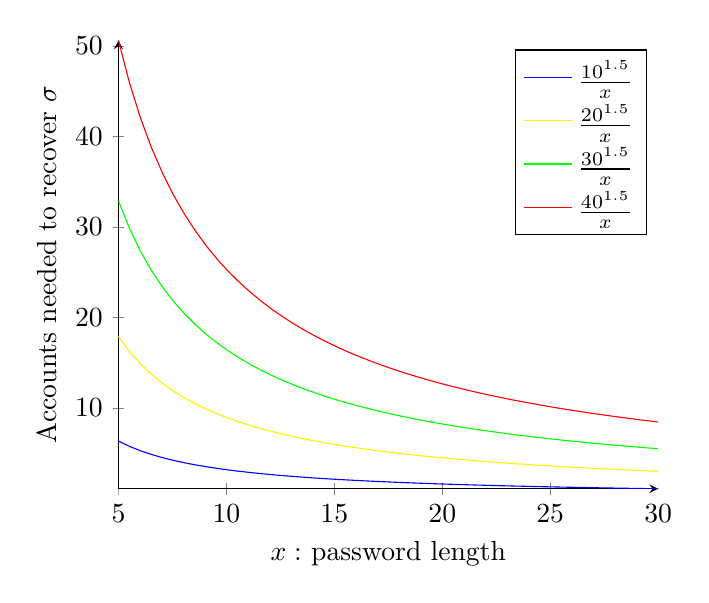
\begin{tikzpicture}
    \begin{axis}[axis lines = left, xlabel=$x: $ password length, ylabel=Accounts needed to recover $\sigma$]
    \addplot[domain=5:30, samples=50, color=blue]{(10^1.5)/x};
    \addlegendentry{$\frac{10^{1.5}}{x}$};
    
    \addplot[domain=5:30, samples=50, color=yellow]{(20^1.5)/x};
    \addlegendentry{$\frac{20^{1.5}}{x}$};
   
    \addplot[domain=5:30, samples=50, color=green]{(30^1.5)/x};
    \addlegendentry{$\frac{30^{1.5}}{x}$};
   
    \addplot[domain=5:30, samples=50, color=red]{(40^1.5)/x};
    \addlegendentry{$\frac{40^{1.5}}{x}$};
\end{axis}
\end{tikzpicture}
\caption{Number of accounts needed to recover the mapping $\sigma$.}
\label{trade-off2}
\end{figure}


\begin{figure}
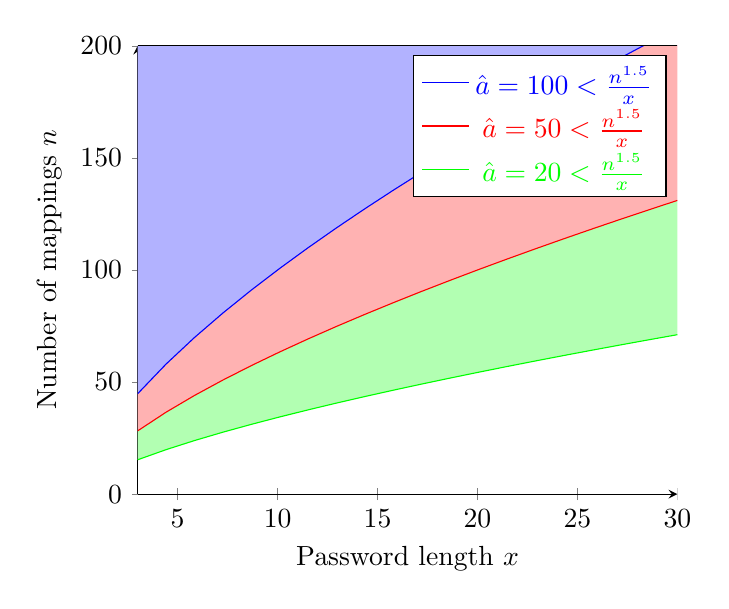
\begin{tikzpicture}
    \begin{axis}[axis lines = left, xlabel= Password length $x$, ylabel=Number of mappings $n$, ymin=0, ymax=200]
   
    \addplot+[name path=A, color=blue, domain=3:30, samples=20, no markers]{(100*x)^(2/3)};
    \addlegendentry[blue]{$\hat a = 100 <  \frac{n^{1.5}}{x}$};

    \addplot+[name path=B, color=red, domain=3:30, samples=20, no markers]{(50*x)^(2/3)};
    \addlegendentry[red]{$\hat a = 50 <  \frac{n^{1.5}}{x}$};

    \addplot+[name path=C, color=green, domain=3:30, samples=20, no markers]{(20*x)^(2/3)};
    \addlegendentry[green]{$\hat a = 20 <  \frac{n^{1.5}}{x}$};

    \addplot+[name path=X, domain=3:30, samples=2, no markers]{200};
    \addplot[blue!30] fill between [of=A and X];
    \addplot[red!30] fill between [of=B and A];
    \addplot[green!30] fill between [of=C and B];
\end{axis}
\end{tikzpicture}
\caption{Inequality plot of 3 different values for $\hat a$}
\label{a-var}
\end{figure}





\section{Practical Usage}\label{usage}
This section illustrates how the HCP scheme works in practice, using the principles described in the previous sections. Before using the scheme a user have to go through a setup procedure involving memorization of a randomly generated mapping as well as setting up all accounts with passwords calculated from challenges. Section \ref{sec-params} discussed how the scheme can be tweaked to fit different needs a user may have, depending on the required level of security and the amount of accounts and passwords a user may have. A summary of the setup and authentication procedures are presented next.
\subsection{Setup procedure.}
\begin{enumerate}
    \item A secret mapping is the first prerequisite required before the scheme can be used. A random mapping of length $n$ is generated from a set of objects chosen by the users, to digits in $\{0,1,\dots,d\}$. Users will typically choose what type of objects to use, this can be an alphabet or a user chosen set of pictures. A system will then choose $n$ of these objects and assign a random digit between $0$ and $d$, $d$ is normally $10$. Algorithm \ref{gen-mapping} shows how the mapping would be generate from a set of objects by assigning random digits to each object. Remember that this mapping function is supposed to only be stored in the memory of the users, and can thus not be evaluated anywhere else than in the mind of each individual user.
    \item Memorization of the mapping is the next, and most costly procedure. Users have to learn the mappings by heart, and be comfortable they will not forget them. After memorizing, the mapping is deleted and not stored anywhere else than in the mind of the users. After finishing this step, there is no way to recover the mapping if users forget it. This might seem like a barrier, but the fact is that the memorization is a one time cost for many users. Active users will naturally rehearse and thus not forget their mappings as long as they keep using the scheme and regularly calculate passwords.
    \item Passwords can now be generated for all the users' accounts. Algorithm~\ref{new-challenge-algo} describes the process of creating new passwords for all accounts. 
    \begin{enumerate}
        \item First users choose the desired length of the password, $t$, to be generated\footnote{In practice this length is not static for all accounts, when adding a new account to the system users will categorize the account, which will decide the length of the password, and thus the number of challenges generated.}. 
        \item $t$ random challenges are generated and shown one by one to the users, which calculate the responses to these. Each of the responses are one character in the new password. 
        \item The calculated password is then sent to the server typically through a ``change password''-form. 
    \end{enumerate}
    \item the same procedure (1-3) can be done for all the accounts users want to include in the password scheme.
\end{enumerate}

\begin{algorithm}
    \caption{Generate mapping $\sigma$.}
    \begin{algorithmic}[1]
        \Require
            \Statex \begin{itemize}
                \item A base $d$.
                \item $O_1,\dots,O_n$ objects, typically letters or pictures.
            \end{itemize}
        
        \For{$i=1 \rightarrow n$}
            \State $k \sim \{0,d\}$
            \State $\vec S \leftarrow (O_i,k)$
        \EndFor
        \Statex

        \Function{$\sigma$}{$O_x$}
            \State search($O_x\quad in\quad \vec S$)
            \State \Return $(O_x, i)$
        \EndFunction
        \Statex
        \State \Return $\sigma$
    \end{algorithmic}
    \label{gen-mapping}
\end{algorithm}
\subsection{Authentication procedure.}\label{subsec:auth}
\begin{enumerate}
    \item Authenticating with a site, which password was previously generated using the scheme, start of by selecting the correct site. The corresponding challenges will then be displayed starting with the first one.
    \item Users calculate the response to each challenge, the same way they did when generating the password. If the calculations are done correctly, the result should be the same.
    \item After calculating the response to all $t$ challenges, the password can be submitted to the server which checks if the hashed value is the same as the stored one. If it is, the user is authenticated.
\end{enumerate}

\begin{remark}
    The notation $f(\sigma(\vec C))$, as used in the algorithms, is equal to the composite function $f \circ \sigma(x_0,\dots,x_{13})$ as used in definition \ref{fo-function}.
\end{remark}

\begin{algorithm}
    \caption{Create new challenge for account $A_j \in (A_1,\dots, A_m)$}
    \begin{algorithmic}[1]
        \Require
            \Statex \begin{itemize}
                \item $t$ desired length of password.
                \item $\sigma$ secret mapping memorized by the user.
                \item $f$ a human computable function.
                \item $O_1,\dots,O_n$ objects, typically letters or pictures.
            \end{itemize}
            
        
        \For{$i=1 \rightarrow t$}
            \State $k \sim [0, n] $
            \State $\vec C_i \leftarrow \{O_k\}^{14} $
        \EndFor
        \Statex
        \State $\vec C \leftarrow (\vec C_1,\dots, \vec C_t) $

        \State \textbf{(User)} Computes $(p_1,\dots,p_t)=f(\sigma(\vec C))$
        \State \textbf{(Server)} Store $h_j = H(p_1,\dots,p_t)$
        \State
        \State \Return $\vec C$
    \end{algorithmic}
    \label{new-challenge-algo}
\end{algorithm}


\begin{algorithm}
    \caption{Authentication process for account $A_j \in (A_1,\dots,A_m)$}
    \begin{algorithmic}[1]
        \Require
            \Statex \begin{itemize}
                \item Account $A_j \in (A_1,\dots, A_m)$
                \item Challenges $\vec C = (\vec C_1,\dots,\vec C_t)$ from account $A_j$.
                \item Hash $h_j$ and hash function $H$.
            \end{itemize}

            \For{$i=1 \rightarrow t$}
                \State Display $C_i$ to the user
                \State \textbf{User} Compute $p_i \leftarrow f(\sigma(C_i))$
                \State
                \Comment $p_i$ is the $i$'th character of the password for account $A$
            \EndFor

            \State $\vec P = (p_1,\dots,p_t)$
            \If{$h_j =H (\vec P )$}
            \Comment \textbf{(Server)} 
                \State Authenticated on account $A_j$
            \Else 
                \State Authentication failed
            \EndIf

    \end{algorithmic}
    \label{auth-algo}
\end{algorithm}



\section{Usability}\label{sec:usability}
Blocki et al. \cite{hcp-blocki} consider three usability parameters defining the usability of a human computable function, namely \emph{calculation time}, \emph{memorizing $\sigma$} and \emph{rehearsing $\sigma$}. In addition to these, another influencing factor is introduced, \emph{failure rate}. This section discusses these requirements and how to influence them.
\begin{itemize}
    \item The effort required to memorize the secret mapping.
    \item The extra rehearsal required of the users to not forget the secret mapping. 
    \item How long it takes a human user to calculate the responses to a set of challenges, eventually producing the password. 
    \item How reliably a human user can calculate password without mistakes.
\end{itemize}
All of these requirements might limit the usability of the scheme, and are thus worth discussing, this project focuses mostly one the last two requirements, related to computation time and failure rates. These parameters are later tested through implementing the scheme as a web app and having participants try it out while timing their efforts. 

\subsection{Memorizing the secret mapping.}
As seen in the previous section, users have to memorize a random mapping from object to digits before starting to use the scheme. This is most likely the biggest and most frightening barrier for any user considering to use the scheme. There are several techniques supposed to help memorizing relations easier, examples are the method of loci \cite{human-memory} which is supposed to enhance memory by visualization. Mnemonic helpers showing objects merged together might help memorize relations as in the case of this project. Blocki et al. \cite{hcp-blocki} propose using mnemonic helpers if the mapping consist of letters to digits. These helpers would typically be a set of pictures showing a visual transition from a letter to a digit. This way might make it easier for users to remember it instead of only being shown ``A=1'' etc. Some user might also feel that it is easier to memorize other things than letters, such as pictures. Users might even get to choose the set of pictures to be used themselves as long as the corresponding digits are chosen at random. 

\subsection{Rehearsing the secret mapping.}
After memorizing the mappings, the users have to rehearse it frequent enough to not forget them. Blocki et al. \cite{naturally-rehearsing} define a model estimating the cost of this rehearsal, the model is described in \autoref{sec:usability-model}. Applying this model to the password management scheme gives insight to how much different types of users have to rehearse. The model predicts how long a user will remember a association between $i$ and corresponding mapping $\sigma(i)$ without further rehearsal. If users are about to forget a mapping according to the predictions, they should be reminded of this. Recall theorem \ref{ERt} and table \ref{users} from \autoref{sec:usability-model}. The formula for $E(ER_t)$ can be used to predict how many extra rehearsals different types of users will be required to do within a given period. \autoref{extra-rehearsals} shows the expected number of extra rehearsals required by the different types of user given the length of the mapping function $n$, during the first year. It is computed using theorem \ref{ERt} with $t=365$ and visitation schedules $\lambda_i$ from each user type as seen in table \ref{users}. For each account $A_i$ a set of public challenges $\vec C_i \in (X_{14})^{10}$ are chosen at random using algorithm \ref{new-challenge-algo}. The expanding rehearsal assumption as defined in \ref{ER} is used, which assumes that for each rehearsal $i$ users does not have to rehearse again for $2^{is}$ units of time. The variable $s$ represents differences between user in terms of memory strength, this experiment uses $s=1$. The values in table \ref{extra-rehearsals} are calculated by generating $100$ samples of $\vec C_i \in (X_{14})^{10}$, then calculating the average expected number of extra rehearsals required by the different user types. 
\begin{table}
    \centering
    \begin{tabular}{ |l|c|c|c| }
        \hline
        User & $n=100$ & $n=50$ & $n=30$ \\
        \hline \hline
        Very Active & $0.396$ & $0.001$ & $\approx 0$ \\
        \hline
        Typical & $2.14$ & $0.039$ & $\approx 0$ \\
        \hline
        Occasional & $2.50$ & $0.053$ & $\approx 0 $  \\
        \hline
        Infrequent & $70.7$ & $22.3$ & $6.1$ \\
        \hline

    \end{tabular}
    \caption{Extra rehearsals required of the users during the first year to remember $\sigma$. Calculated using definition \ref{ERt} with $t=365$ and visitation schedules as in table \ref{users}~\cite{hcp-blocki}.}
    \label{extra-rehearsals}
\end{table}

\par The results in table \ref{extra-rehearsals} clearly demonstrates that the HCP scheme does not require much rehearsal at all if used frequently. In fact, for very active, typical and occasional users, memorizing the mapping is a one time cost. After memorizing it at the beginning, using the scheme will provide enough natural rehearsal to maintain the mapping in memory. 
When users compute the response to a challenge $\vec C$, they will have to recall the mapping of up to $5$ ($(\sigma(x_{11}), \sigma(x_{10}), \sigma(x_{12}), \sigma(x_{13}),\sigma(x_j)$) values of $i$ for each character of the password. A password length of $10$ would yield recalling, and thus rehearsing, $50$ values of $i$. The same trade-off as discussed in \autoref{sec-params} can be observed here. The more complex the mapping is (larger values of $n$), the more effort is required when memorizing, but no extra rehearsals are necessary even with a larger number of mappings.

    \subsection{Computation Time and Failure Rates.}\label{computation-time}
The final requirement which may limit the usability of the scheme is calculation time. If users can not compute the response to a challenge correctly in a reasonably short amount of time the scheme would not be usable. How much time users can tolerate is of course individual, but a too long computation time will directly effect the usability. In addition to the time spent calculating, it is important that the users are able to consistently compute the correct responses. If the failure rate is too high, in respect to the password length, the scheme will not function at all. It is thus more important to have a low enough failure rate than a short calculation time.


\subsubsection{Improving Usability.}\label{improving-usab}

\par To make the computation as easy as possible the challenges are presented to the users in a practical way, facilitating fast and reliable calculation. Using the human computable function from definition \ref{fo-function}, a challenge $C = (x_0, x_1,\dots, x_{13})$ could be displayed as shown in \autoref{challenges}. \\ 
\centerline{ $f\circ \sigma(x_0,x_2,\dots,x_{13}) =$} \\
\centerline{$\big(\underbrace{\sigma ( x_{ (\underbrace{\sigma(x_{11}) + \sigma(x_{10}) )\quad mod \quad 10}_\text{Step 1, 2, \& 3}} )}_\text{Step 4 \& 5} \underbrace{ +\sigma ( x_{12} ) + \sigma( x_{13} )\big)\quad mod \quad 10 }_\text{Step 6 \& 7}$ }. 

To evaluate a challenge using this function and the layout template from \autoref{challenges} users goes through the following steps:
\begin{enumerate}
    \item Recall the mapping $x_{10}$
    \item Recall the mapping $x_{11}$ 
    \item Add the values from the two previous steps $j = \sigma(x_{10}) + \sigma(x_{11})$.
    \item Locate the element $x_j$ from the table.
    \item Recall the mapping $\sigma(x_i)$.
    \item Recall the mapping $\sigma(x_{12})$ and add this to the previous value, $z = \sigma(x_i) + \sigma(x_{12})$.
    \item Finally recall the mapping $\sigma(x_{13})$ and add it to the previous value, obtaining the final sum $y = z + \sigma(x_{13})$k.
    \item $y$ is the response to challenge $C$.
\end{enumerate}


\begin{table}[h]
    \centering
    \begin{tabular}{|c c|c|c|}
        \hline
        $x_{10}$ & $x_{11}$ & $x_{12}$ & $x_{13}$ \\
        \hline \hline
        \multicolumn{2}{|c|}{$0:x_0$} & \multicolumn{2}{|c|}{$5:x_5$}\\
        \multicolumn{2}{|c|}{$1:x_1$} & \multicolumn{2}{|c|}{$6:x_6$}\\
        \multicolumn{2}{|c|}{$2:x_2$} & \multicolumn{2}{|c|}{$7:x_7$}\\
        \multicolumn{2}{|c|}{$3:x_3$} & \multicolumn{2}{|c|}{$8:x_8$}\\
        \multicolumn{2}{|c|}{$4:x_4$} & \multicolumn{2}{|c|}{$9:x_9$}\\
        \hline 
    \end{tabular}
    \caption{Layout template for displaying challenges.}
    \label{challenges}
\end{table}


\par Each step depends on at most two earlier steps, allowing users to do the calculation without having to store more than two values in memory at any time. After finishing steps 1-3 they will only keep one value in memory, the previous intermediate results are now irrelevant and can be forgotten. 

\begin{example}
    \autoref{challenge-example} shows the same layout using example objects. The example challenge is $C = \{A, B, C, D, E, F, G, H, I, J, K, L, M, N\}$. Let the mapping function $\sigma$ be the position in the alphabet $\bmod 10$, $\sigma(A)=1, \sigma(B)=2, \sigma(J)=0$ etc. The evaluation of this challenge would be the following.
    \begin{enumerate}
        \item $\sigma(K) = 1$, $\sigma(L)=2$ (K is the $11$th letter in the alphabet, thus $11 \bmod 10 = 1$)
        \item $(11 + 12) \bmod 10 = 3$
        \item $x_3 = D$
        \item $\sigma(D) = \underline{4}$ , $\sigma(M)=\underline{3}$, $\sigma(N)=\underline{4}$
        \item $(4 + 3 + 4) \bmod 10 = \underline{\underline{1}}$

    \end{enumerate}

    
    \begin{table}[h]
        \centering
        \begin{tabular}{|c c|c|c|}
            \hline
            $K$ & $L$ & $M$ & $N$ \\
            \hline \hline
            \multicolumn{2}{|c|}{$0:A$} & \multicolumn{2}{|c|}{$5:F$}\\
            \multicolumn{2}{|c|}{$1:B$} & \multicolumn{2}{|c|}{$6:G$}\\
            \multicolumn{2}{|c|}{$2:C$} & \multicolumn{2}{|c|}{$7:H$}\\
            \multicolumn{2}{|c|}{$3:D$} & \multicolumn{2}{|c|}{$8:I$}\\
            \multicolumn{2}{|c|}{$4:E$} & \multicolumn{2}{|c|}{$9:J$}\\
            \hline 
        \end{tabular}
        \caption{Layout template for displaying challenges.}
        \label{challenge-example}
    \end{table}


\end{example}

\paragraph{Classification of accounts.}
Section \ref{classification} discussed how different accounts should be treated differently depending on the consequences of compromise of the accounts. This can be utilized to limit the number of single digit challenges a user needs to calculate when logging into each account. When adding an account to the system users have to classify the account in terms of how big consequences a breach would have. This way the users are in control of how much effort is spent calculating passwords versus how strong the passwords are. This will essentially lower both the average total calculation time and attempts needed to calculate each password. 

\par This chapter has presented the ideas behind the HCP management scheme. It has shown how the scheme works with a secret mapping memorized by the users and a human computable function, which together allow users to compute passwords from challenges stored in persistent memory. Algorithms describing the procedures has been shown and described, as well as discussing the usability challenges of such a scheme.


\cleardoublepage
\chapter{Application}\label{app}
This chapter will describe how browser extensions are built in google chrome, focusing on architecture and security features. Browser extensions can be utilized to build an application implementing "human computable passwords" as described in \autoref{ch:hcp}. The scheme is different from other traditional password managers since it does not \emph{store} the password, but challenges \emph{helping} the user to remember strong passwords. The idea by using browser extensions to implement this is to have an extension monitor the password fields of the sites a user visits and update the challenges depending on the current state of the active site. This technique will be described and a prototype extension demonstrated. 
\section{Browser Extensions}\label{browser-extensions}
Modern computer users shift towards doing more and more work through their web browsers. Web applications have become popular due to the ubiquity of browsers, thus allowing web apps to run anywhere. A web app can run at any platform running a web browser, allowing the application to run on multiple platforms as well as different devices. Updates can be applied quickly without having to distribute patches to a possibly huge amount of devices.
\par Browser extensions add additional features to the web browser allowing the user to tweak the experience of the web pages visited. Typical examples are extensions adding to, or tweaking already present features of the browser such as changing how bookmarks are managed, or adding additional features such as blocking advertisements. Lately browser extensions have been extended even further allowing standalone applications to be developed running as native applications \footnote{A new breed of Chrome apps, \url{http://chrome.blogspot.no/2013/09/a-new-breed-of-chrome-apps.html} - accessed: 2015-03-02}. This allows developers to create desktop apps using the same technology as in web apps, mainly HMTL5, Javascript and CCS.
\par This chapter will present Google chrome browser extensions, including architecture and security mechanisms.

%This project will utilize chrome extensions to create a password manager running in the browser. 
%The user interface will be in a panel spawned by a browser action activated when the user click the icon in the navbar. 
%The user interface is built using the open-source web application framework AngularJS \cite{angularjs}, storage is done using the chrome local storage API.

\subsection{Extension Security}\label{extension-sec}
\par Browser extensions introduce some security concerns which must not be forgotten while developing applications using this environment. Chrome extensions run in the browser with access to both the \gls{dom} of the active page as well as the native file system and connected devices. The overall architecture of the application is summarized in \autoref{extension-architecture} and described in the chrome extensions documentation \footnote{What are extensions?, \url{https://developer.chrome.com/extensions/overview} - accessed 2015-03-02}. This section will describe the architecture considering security concerns relevant when developing chrome extensions which handle sensitive data such as passwords.

%The extension core consist of the actual application interface visible to the user as well as long running background jobs and business logic. The background page can be used to spawn panels or popups, and has access to browser APIs.  The extensions is activated through a icon in the browser navbar as seen in \autoref{extension-ux}. Clicking the icon typically spawns a popup or a panel to interact with the user. In addition to the core, each extensions can have content scripts which has access to the content of the current active web page, and can monitor and alter \gls{dom} of this. 


\begin{figure}[h]
   \fbox{\includegraphics[width=\textwidth]{chrome-extension-architecture} }
    \caption{Chrome extension architecture.}
    \label{extension-architecture}
\end{figure}

\par Earlier extensions written for IE and Firefox ran in the same process as the browser and shared the same privileges. This made extensions an attractive entry point for attackers, since a buggy extension could leave security holes leaking sensitive information or even provide an entry point to the underlying operating system. For these browsers several frameworks for security have been proposed \cite{firefox-ie, js-info-flow}, trying to mitigate vulnerabilities is browser extensions. The chrome extensions architecture is built from scratch with security in mind. Chrome uses a permission system following three principles \cite{liu-chrome}; \emph{least privileges}, \emph{privilege separation} and \emph{process isolation}. 

\paragraph{Least privilege} specifies that extensions should only have to privileges they need functions, not share those of the browser. The privileges of each extension are requested in the \emph{manifest} file \footnote{Manifest file format, \url{https://developer.chrome.com/apps/manifest} - accessed 2015-03-04}. This json file needs to be included in all chrome extensions, and consist of all the permissions needed by the extension as well as some meta data and version information. This is done to prevent compromised extensions from exploiting other permissions than those available at runtime. An example of a manifest file can look like this: 

\begin{verbatim}
{
    "name": "Example extensions",
    "description": "An example extensions to demonstrate how the
                    manifest file works.",
    "version": "1.2",
    "manifest_version": "2"
    "background_page": "main.hmtl",
    "permissions": [
        "bookmarks",
        "storage",
        "https://*.ntnu.no"
    ]
}
\end{verbatim}
This extension has specified access to the bookmarks API, chrome local storage and all sub domains of ntnu.no. Extensions can request different permissions in the manifest file including web site access, API access and native messaging. If an extension contains weaknesses it will not compromise any other parts of the system not covered by the specified privileges. For the least privileges approach to work properly each developer should only request the permissions needed, Barth et al. \cite{protecting-browsers} examined this behavior and concluded that developers of chrome extensions usually limit the origins requested to the ones needed. 

\paragraph{Privilege separation.} Chrome extensions are, as mentioned, divided into components; content scripts, extension core and native binaries. The addition of native binaries allows extensions to run arbitrary code on the host computer, thus posing a serious security threat. This project does not use this permission, this component will thus not be mentioned from now on. 
\par \emph{Content scripts} are javascript files allowing extensions to communicate with untrusted web content of the active web page. These scripts are instantiated for each visited web page and has direct access to the \gls{dom} of these, allowing both monitoring and editing of DOM elements. To be able to inject content scripts to a visited page, the origin of the site has to be added to the manifest file. Other than this permission, content script are only allowed to communicate with the extension core. It is important that the privileges of these scripts are at the minimum level since they are at high risk of being attacked by malicious web sites \cite{chrome-extension-dangers}, due to the direct interaction with the \gls{dom}. 
\par The \emph{extension core} is the application interface responsible for interaction with the user as well as long running background jobs and business logic. The core is written in HTML and javascript and is responsible for spawning popups and panels, as well as listening for browser action. The typical way to activate a extensions is by clicking an icon in the navigation bar, which then activates either a popup or a detached panel. The core is the components with the most privileges as it does not interact with any insecure content directly, only through direct messaging to a content script or using http requests if the target origin is defined in the manifest. 
\par In addition to this the core has access to the extension APIs, these are special-purpose interfaces providing additional features such as alarms, bookmarks, cookie and file storage. The APIs are made available through the manifest file and only those specified there can be used. \autoref{extension-ux} illustrates the interaction between the background page, content scripts, panels and active web page. The information flow starts by clicking the extension's icon in the navigation bar which launches the background page spawning a panel in the browser. A content script is injected in the current web site (google.no in the example), the script now have access to the DOM of this site and can communicate with the background which in turn can update the panel. 


\begin{figure}[h]
    \fbox{ \includegraphics[width=\textwidth]{chrome-extension-ux} }
    \caption{Chrome extensions browser action and content scripts.}
    \label{extension-ux}
\end{figure}

\paragraph{Process isolation} is a set of mechanisms shielding the component from each other and from the web. Usually when javascript is loaded from the web the authority of the script is limited to the origin from where the script is loaded \cite{protecting-browsers}. Since the scripts used by the extensions are loaded from the file system, they do not have a origin in the same sense, and thus need to be assigned one. This is done by including a public key in the url of the extension, allowing a packaged extension to sign itself, freeing it from any naming authority or similar. The public key also enables usage of persistent data storage, since the origin of the extension can stay the same throughout updates and patches. This wouldn't be possible otherwise since the chrome local storage API relies on origin. \todo{more details}
\par The different components also run in different processes. The content scripts are injected and ran in the same process as the active web page, while the core run in its own process started when the extension is initiated. \todo{paragraph not finished. Cross-origin js and malicious web site operators.}
\par Finally content scripts are ran in a separate javascript environment isolating it from the possibly insecure environment of the web site. The environment of the content scripts are called isolated world, which in practice is a separate set of javascript objects reflecting the ones of the underlying DOM of the web page. This means that the content script can read and edit the DOM of the page it is injected into, but not access variables or javascript functions present in the web page. Both the page and the content scripts sees no other javascript executing in their own isolated world, but they share the same DOM \footnote{Content Scripts, \url{https://developer.chrome.com/extensions/content_scripts} - accessed: 2015-03-05}.


\section{Human Computable Passwords Chrome Extension}
\todo[inline]{Present the idea of why and how a chrome extensions can be built to realize the scheme}
Chrome extensions are very useful in that they can be ran from any computer with Google chrome installed, thus on any operating system and on any computer. An extension makes it possible to run applications while browsing the web, which in the case of an password management scheme is very useful. An application meant to help the user recall complex passwords should preferably be visible simultaneously with the password field. The most popular password management software today are usually either web applications, mobile applications or native desktop applications\footnote{Five Best Password Managers. \url{ http://lifehacker.com/5529133/five-best-password-managers }}, some of these might include plug-ins such as browser extensions. All of these password managers are reliably storing all the passwords as described in \autoref{subsec:pms}, then they are either auto-filled into the login fields or through copy pasting manually. 
\par This section will present the design and prototype implementation of the human computable password scheme (\autoref{ch:hcp}, \cite{hcp-blocki}. The design evolves around the fact that the scheme does not have to store anything securely, it is though important to make it as easy as possible for the user. The architecture will be similar to the one explained in \autoref{browser-extensions} using content scripts to monitor the password fields of the active browser session. The user interface will be presented through a "panel" in the browser. Panels are windows that stays in focus will interacting with other windows or applications \footnote{"Panels"- The Chromium Project. \url{https://www.chromium.org/developers/design-documents/extensions/proposed-changes/apis-under-development/panels}}. 




\subsection{Applications Design}
\todo[inline]{Relate the ideas and architecture presented in the previous section. Explaining how content script and local APIs will be use used to provide an extension supporting the scheme }
\todo[inline]{Models of how the extensions will look including both user interface and architecture}
The extension implementing human computable passwords \ref{ch:hcp} will be an extensions helping the user with storing and managing of challenges for different accounts. The generation of secret mappings will not be part of the application, this should be done through a separate program on the user's local computer. Such a program would follow \autoref{gen-mapping}. The requirements for the extension are the following:

\begin{itemize}
    \item Provide an user interface making it easy for the user to display challenges for different accounts.
    \item The application should keep track the active site, displaying challenges for the correct site without user interaction.
    \item Add new sites to the system easily. 
    \item Displayed challenge should update while typing the password.
    \item The user should be able to type his password directly in the password field of the active site.
    \item If the user is about to forget a secret mapping, according to the usability model \ref{sec:usability-model}, the application should notify about it and advice the user to rehearse.
\end{itemize}


\subsubsection{AngularJs}
The front-end is built and updating using AngularJS\footnote{AngularJS, \url{https://angularjs.org/}}, which is a open source, client-side javascript framework. Angular is built using a variation of the model-view-controller architecture \cite{mvc}, though the creators of angular states that angular is a model-view-whatever framework\footnote{Model-View-Whatever - \url{ https://plus.google.com/+AngularJS/posts/aZNVhj355G2 }}, point being that what the architecture is called isn't important. The \emph{view}s in angular is templates written entirely in HTML making it easy read and update. The \emph{controller} contains all the business logic used by the view. The views and controllers are connected using a shared object called \emph{\$scope}, variables or functions on this object is usually defined in the controller and accessed by the view by using double curly brackets in the view (e.g. \{\{name\}\} to access the name variable on \$scope). Figure \ref{angular-data-binding} shows how scope is used to share variables between the controller and the view. 
\par Services in angular are reusable business logic which can be used independent of the views and controllers\footnote{Services - \url{https://docs.angularjs.org/guide/services}}. Services will be used to handle variables which are shared between the view and the content scripts (explained later).

See "Angular Essentials - Rodrigo Branas"\cite{angularjs-book} for a step-by-step introduction to AngularJS.

\begin{figure}[h]
    \includegraphics[width=\textwidth]{angular-data-binding} 
    \caption{Angular data binding with controller, view and scope. Figure from angular developer guide.}
    \label{angular-data-binding}
\end{figure}


\par The main benefits of using angular in this project is the data-binding which makes it easy to update the HTML shown to the user. The extension will take advantage of this when updating the challenges seamlessly while the user calculates his password.

\subsubsection{Chrome Storage.}
\emph{Local storage\footnote{Local storage - \url{ http://diveintohtml5.info/storage.html }}} is a way for applications to store data persistently and securely in the browser of clients. It is meant as an improvement of cookies which is the usual way of storing user data across sessions. The biggest problem with cookies is that they are sent with every HTTP request and thus slow down the applications using them. Local storage allows applications to store (key, value)-pairs in the browser. 
\par \emph{Chrome storage} is close to the same as local storage, differences being that chrome local storage allows applications to store data in what is called "chrome.storage.sync". This specific storage saves data locally, but also syncs it with the currently active chrome account, thus allowing a user to log into his account in any chrome browser and access the same application data. Chrome storage also allows storage of objects compared to local storage which only allows storing strings. This project will use chrome storage to persistently store challenges across sessions, and also provide backup. This way each user will be able to keep challenges for all their account within the storage of their google account. This is a important feature since it allows access to the challenges from remote locations as well.

\subsubsection{Content Scripts.}\label{cs}
Content scripts are javascript files running in the context of the active web page, as browsed by the user. These scripts has direct access to the content of the active site and can thus monitor and attach event listeners.The content scripts are isolated from the extension itself as describe in \autoref{extension-sec}, thus protecting the extension from possibly harmful sites trying to exploit weaknesses in the content script. Because of this the content scripts has to communicate with the extension through google chrome's built-in message passing system. Chrome message passing\footnote{Chrome message passing - \url{https://developer.chrome.com/extensions/messaging}} allows script to listen for and respond to messages. One side set up an event listener listening for messages, when a message is sent from the other side this event triggers and the message can be received and parsed. 
\par The content scripts and the message passing system are the only likely points of attack for adversaries. The content script can monitor the value of the password field and thus, in theory, steal these if a malicious script was able to trick it into leaking these. The communication channel is not particularly prone to attacks since even if an adversary eavesdropped all data sent on it, the only information leaked would be the current length of the password. It is though important that the design is like this since the mistake of sending the whole password string, which might seem like a solution, would be potentially dangerous. 
\par Typical usage of content scripts in this application will be to attach event listeners to the password fields of the pages visited by the user, and message the extension when the value of the password field changes. When a change happens, the content script send a message containing the current length of the typed password, so that the extension can display the correct challenge. In example if the user has entered 4 characters of his password the extension should display the 5th challenge etc. The content script also keep the extension updated on the URL of the current page, by sending a message every time a page is loaded. The extension then displays the challenges corresponding to the password of that site. If the site does not have challenges stored by the application, the user can generate new ones and store these in the system through clicking a button.  

\subsection{User interface}
The user interface will be very simple, there will be two possible screens displayed to the uses. Either challenges associated to the current page will be shown, or a dialog asking the user to generate new challenges. The most important feature of the user interface is that it will automatically update depending on what site the user is currently browsing, and display the correct challenge when typing passwords. Wireframes illustrating the page schematics of the extension are shown in figures \ref{add-new-screen} and \ref{challenge-screen}.

\begin{figure}[h]
    \centering
    \begin{subfigure}[t]{0.49\textwidth}
        \centering
        \includegraphics[width=\textwidth]{wireframe} 
        \caption{Screen seen by the user when launching the extension when visiting a page that is not stored in the system.}
        \label{add-new-screen}
    \end{subfigure}
    \hfill
    \begin{subfigure}[t]{0.49\textwidth}
        \centering
        \includegraphics[width=\textwidth]{wireframe2} 
        \caption{Screen seen by the user when loading a site with challenges stored in the system. }
        \label{challenge-screen}
    \end{subfigure}
    \caption{Wireframes illustrating the page schematics of the extension.}
    \label{wireframes}
\end{figure}

\subsection{Implementation}
\todo[inline]{Present the actual design and choices made}
\todo[inline]{Demonstration of how the extension works in practice.}
\todo[inline]{Walkthrough of setting up/authenticating with an account using the scheme and the extension. }
The implementation follows the design described in the previous section, this section will present how the extension are implemented and present the actual extension.


\subsection{Architecture}
\par \autoref{class-diagram} shows the complete architecture of the system.
 The content script attach an event listener to the password field of the active site. If the content of the password field changes, the script sends a message using chrome message passing containing the current length of the password. The controller receives the new password length through the data service, and update the challenges displayed to the user. The data service is also responsible for updating the URL field accessible to the controller.

\begin{figure}[h]
    \centering
    \fbox{ \includegraphics[width=\textwidth]{class-diagram} }
    \caption{Class diagram of the human computable passwords chrome extension.}
    \label{class-diagram}
\end{figure}
\par The classes seen in figure \ref{class-diagram} are all represented in the implemented version of the extension. The construction and responsibilities of the classes are summarized in the following list.
\begin{itemize}
    \item[Controller] is responsible for the business logic related to the information shown to the user in the extension. The controller first tries to load the user data stored in chrome storage, if no user has been created, typically if it is the first time the extension is loaded, a new user is created. In this project the controller also injects a set of dummy-data for the purpose of demonstration, in a real world scenario sites would have to be added through the "add new site"-screen.
    \item DataService
    \item ChromeStorage
    \item Content script   See \autoref{app:content-script} for the content script file with a brief description of the code. 
    \item Main.html

\end{itemize}


\subsection{Discussion}
\todo[inline]{Discuss how and why using an extension instead of a typical web or mobile application is more usable etc. }








\cleardoublepage
\chapter{Usability Experiment}\label{ch:experiment}
This chapter presents the design and execution of an experiment trying to measure  the performance of the HCP scheme. The experiment is designed as a web application implementing the scheme, allowing participants to test how the scheme would work in practice while measuring how fast and reliable the computation is performed. The application acts as both a demonstration app and a tool for gathering performance data. It has four sections designed to help the participants understand the scheme and get familiar with the computation technique. First, a demonstration video is shown explaining how to compute a password from a challenge, then users are asked to enter some demographic data. Next is the practice section, where users are supposed to practice doing the calculation until feeling comfortable solving challenges without error. Finally is the experiment part, where the calculations are timed and correctness monitored. After finishing the calculations user submit the data and can choose to continue doing more experiments now, or later.
\section{Experiment Objective}
The goal of the experiment is to measure how hard it is for a user to learn the scheme, i.e. how fast and reliable users do the calculations. The experiment measures the calculation times of the participants, and also monitor their progression after several trials. Users should also be able to calculate passwords without too many mistakes. The failure rate is maybe the most important variable to measure; if a user averages more than one mistake for each password calculated the scheme would not work in practice, since most passwords calculated would be wrong. 
\par It is important to note that this project does not see the HCP scheme as a replacement for the widely used standard password managers. It is regarded as a solution for users interested in a secure and reliable way of keeping track of strong passwords, without having to trust a password management service or application. This experiment tests if it is even possible, for users willing to go through the trouble of learning a secret mapping, to use the scheme as an everyday solution.

\par The objectives of the experiment can be summarized as the following.
\begin{itemize}
    \item Measure the average calculation times, both for each participant and for the whole population.
    \item Measure how much users improve after several trials.
    \item Measure the average failure rate for each participant.
\end{itemize}


\section{Method}
The experiment does not try to test any preset hypothesis as it is not clear what to expect regarding either of the tested values. It is not known how hard it is do to the calculations, neither regarding calculation times or failure rates. The results of the experiment does not give an answer, but rather a basis for further data collection through larger scale experiments, for example using crowd sourcing or social medias.

\par Exploratory data analysis (EDA) was introduced by John W. Turkey~\cite{turkey} and involves analysis of data without a prior hypothesis to test. The technique promotes exploration of data to possible find characteristics not previously considered, and essentially suggesting hypotheses to be tested in later surveys or experiments. Velleman and Hoaglin~\cite{exploratory-analysis} describe EDA as a contrast to the formal scientific method involving stating a hypothesis, collecting data and applying a statistical test of the hypothesis. EDA often involves making graphical representations of the data, and then trying to find interesting characteristics and relations. EDA does not conclude with a hypothesis test based on the collected data, but is the first step of an iterative process trying to reveal facts. 

\begin{remark}
 The project does not store any personal information about the participants, and is thus not subject to notification to the "Norwegian Social Science Data Service"\footnote{Is my research project subject to notification? - \url{http://www.nsd.uib.no/nsd/english/pvo.html}}. The experiment only records an anonymous id plus the experiment results consisting of computation time and correctness of the calculations done. Some demographic data is also recorded (age, area of study), but the data can not be connected to person and are thus not regarded as personal information.
 \end{remark}

\par After conducting the experiment, the data is examined and significant characteristics discussed. There are some obvious parameters to explore, including means and standard deviation of the calculation times and failure rate, as well as how these change with practice. 

\par The usability of the scheme directly relies on the calculation time and failure rate as discussed in section \ref{sec:usability}. This can be discussed further after obtaining some numbers giving a picture of what is normal and possible in terms of speed and reliability.


\par A result showing that more than 95\% of all calculations are correct would be promising, since it would mean that approximately 60\% of the passwords calculated would be correct, given length 10 passwords. If the failure rate is significantly worse, the scheme would more often than not be useless since most users would obtain a faulty password when trying to log in. The conclusion of the experiment presented in this project will either way have to be tested more thoroughly, possibly using the same experiment setup or preferably with a throughly random mapping as well. 



\section{Experiment Setup}
The experiment presents and demonstrates the calculation technique to the users, which then is given a chance to practice until fairly familiar with the mechanics. Finally users are asked to calculate a complete password challenge, from which the time spent on each single digit challenge is recorded, as well as if the calculation was correct or not. The practice section allows users to learn through trial and error, using backspace to go back and forth between challenges while also given feedback on the correctness. The experiment view on the other hand does not give any feedback and does not allow user to go back after entering a character. This is done to make sure all mistakes are recorded, even if it is only a miss click. 
\subsection{Secret mapping} The biggest decision made in regards to the experiment design was how to simulate the operation ``recall'' i.e. recalling from memory. It would not be feasible to ask all the participants to memorize a secret mapping beforehand as this would make it very hard to find volunteers. The chosen solution to this problem is to include a ``cheat sheet'' in addition to the displayed challenges, i.e. a list of object to digit mappings shown separately but in the same view as the challenge.
\par After some testing it became apparent that there was a big difference between recalling from memory and actually ``reading'' from a list, which this approach eventually is. To make the operation more similar to the desired recall operation, the mapping was changed from random alphabet positions (e.g A=1, B=2, C=3). This way one does not always have to read in the table to know the mapping. Most users will be able to know instantly what the mapping for at least the first and eventually, after some practice, all the letters, much easier than with a random mapping. The is the closest way of mimicking the actual operations of the scheme without having the participants memorize an actual mapping. It is not in any way certain that this shortcut reflect the real world act of recalling from memory, but it is assumed to be ``close enough'' for the experiment. 
\begin{remark}
The author of this project did memorize a mapping of both 10 and later 20 mappings without significantly different calculation times compared to using the alphabet positions.
\end{remark}

\subsection{Participants}
The participants for the experiment were chosen mostly from people known by the author, this limits the number of participants somewhat. This was done to ensure the quality of the data samples. The experiment could have been distributed through crowd sourcing services or social media, probably increasing the number of participants drastically. The problem with this approach, and the reason for not doing it, is that the experiment requires absolute concentration which can not be assured from ``casual'' participants accessing the experiment through a link posted on facebook. Since every participant calculates 10 single digit challenges for each trial of the experiment, there is still a decent amount of data samples, even with relatively few participants. 
\par Even if the experiment might be limited by the number of participants, the results are still considered to be interesting. Since the scheme tested is not supposed to be a widely-deployed password manager, it might be sufficient if the experiment can show that some users are able achieve what is considered sufficient usability. It should also be noted that most of the participants are regarded above average in mathematics. This might be a strength or a weakness of the experiment as it does not represent a wide range of the population, but the calculation times should at least be stronger than average.


\section{Web Application}
The experiment application is similar in design to the Chrome extension presented in \autoref{app}, but implemented as a web application. It is implemented using the AngularJS framework (as described in \autoref{app}) and a mongoDB\footnote{mongoDB - \url{https://www.mongodb.org/}} database to store the results, a cookie in the users' browser is used to keep track of users across trials. 

\par The application consists of four sections to flip through, with the last one being the actual experiment. First, users are presented with a video demonstration of the scheme and instructions on how to calculate passwords. The slides used to instruct users can be seen in \autoref{demo-slides}. After watching the demo, users are asked to enter some demographic data (age and occupation). Next, is a section which looks the same as the experiment, but without the actual recording of data, this is the practice section. The purpose of this section is to give users a chance to verify that they have understood the scheme and are actually able to calculate passwords. When users are ready to start the experiment, they can continue on to the actual experiment, which is the final view. The experiment is exactly like the practice section, without response on correctness and redo capabilities, with backspace deactivated. The first sample of the experiment is not counted towards the results, allowing users to get ready and start when they feel like it. 


\par Section \ref{computation-time} discusses how a single digit challenge can be presented to users in a logical way, possibly making it more efficient to calculate. The experiment uses a similar layout to the one shown in \autoref{challenges} and also as in the Chrome extension in chapter \ref{app}. The challenges update in the same way as in the chrome extension so users should be able to calculate the responses continuously. The calculation time is recorded for each single digit challenge computed, together with a boolean value representing if the result was correct or not. 
\par Figure \ref{complete-experiment} shows the screen after completing a trial of the experiment, next users will push the submit button and the sample would be saved in the database together with a random identification stored in a cookie in the users' browsers. Users can then redo the experiment several times keeping the same id, making it possible to track each participant's development.

\begin{figure}[h]
    \includegraphics[width=\textwidth]{complete-experiment}
    \caption{The experiment screen seen after completing an experiment sample, ready to be submitted.}
    \label{complete-experiment}
\end{figure}

\par As for the storage of results a noSQL database called MongoDB is used. After completing a trial of the experiment a Javascript object is stored in the database, \autoref{db-obj} shows an example of this object. Note the \emph{hcp\_id} field which is fetched from a cookie in the participants' browsers, making it persist across several trials. 

\par The views of the web application can be seen in \autoref{experiment-views} or by visiting the hosted experiment site at \url{hcp.sp1nakr.com}.

\begin{table}
\begin{tabular}{|c|c|}
    \hline
    hcp\_id & 1b7aa17ea0  \\ \hline
    occupation & Technology student \\ \hline
    age & 27 \\ \hline
    results & $[1,1,1,1,1,1,1,1,1,1]$ \\ \hline
    calcTimes & $[12.047,7.115,8.022,9.283,10.544,8.807,9.925,9.78,7.11,8.187]$ \\ \hline
\end{tabular}
\caption{Experiment object after completing a trial, as stored in the database.}
\label{db-obj}
\end{table}

\section{Results}

This section presents the results of the conducted experiment and investigate the characteristics of the data recorded. The focus is on the calculation times and failure rates, which both are important factors in the resulting usability of the scheme, as discussed in \autoref{sec:usability}.
\par The observations made are not necessarily representative for all users, because of the relatively small number of samples ($467$ single digit challenges), but it is still interesting to investigate the consequences of the results. Even if the results show that the scheme achieves a lower level of usability than what are considered acceptable, it might still function well for some users with the right amount of practice. The limitations of the experiment is discussed, in addition to results and the consequences of these.

\subsection{Calculation times.}
How fast a user is able to calculate the response to a single digit challenge is a concrete measure of the usability of the scheme. Figure \ref{histo-calctimes} shows the distribution of calculation times of all the experiment samples, the calculated average off all the $467$ trials are $10.296$ seconds. The median value is $9.406$ with standard deviation of $3.64$ which also can be observed in the figure. 
\par Recall conjecture \ref{conjecture1} from \autoref{human-func}. The function $f$ (see definition \ref{fo-function}) used in this project is $(P,9,3)$-computable. The conjecture then defines the variable $\gamma_H$ for user $H$ as {\Large $\gamma_H = \frac{\hat t}{9}$}. 
\par The average $\gamma$ of all the participants are $\tilde \gamma = \frac{10.104}{9} = 1.227$. This is slightly higher than the $7.5$ seconds ($\gamma_H \le 1 $) Blocki~\cite{hcp-blocki} predicts that users with moderate mathematical backgrounds should achieve. It is still not unreasonably high, and should not be a direct hindrance. Calculating a 10 character password would for example take $10 \cdot 10 = 100$ seconds, just above $1.5$ minutes, to calculate, 15 character would take $2.5$ minutes. On average spending 2-3 minutes calculating a password might seem like a lot, but users concerned about the security of their accounts, might be willing to make this trade-off. Especially if users are worried about putting passwords in the hands of a online service to store persistently (e.g. \emph{lastpass.com}), might be willing to put quite some time into calculating passwords instead.
\par It is also relevant to study the evolution of each user in terms calculation times. Figure \ref{scatter-regression} illustrates the average calculation time for each $i$th trail per user. $i=1$ represent the average of the first calculation done by each user, $i=2$ the second calculation etc. The figure clearly illustrates that the averages decrease with practice. This could have been expected, since users will be more and more familiar with the calculation procedure for each trial. The consequence of this observation is that the average calculation time, and consequently $\gamma$, would be significantly lower if the participants got more practice with the scheme before their results was recorded. Each participant averaged $33$ samples each, so it is not feasible to e.g. calculate the average after removing the 20 first calculations from each participant, as this would leave very few trials. The important goal of the experiment is though not to find an accurate average calculation time, but to verify that $\gamma_H \le 1$ is achievable. It seems that the average most likely is somewhere between 9 and 11 seconds, depending on how long users have been using the scheme, which is not severely limiting.
\par Figure \ref{user-regression} and table \ref{tbl:bestuser} shows the 7 participants with the most samples, the same effect can be observed, all except from one participant have a downward going trend (see SCT in table \ref{tbl:bestuser}).

\begin{table}[h]
    \centering
\begin{tabular}{|c|c|c|c|c|}
    \hline
     SMP & MCT & SDCT & SCT & MFR \\ \hline \hline
    $72$ & $9.02$ & $2.38$ & $-0.015$ & $0.0695$\\\hline
    $36$ & $10.06$ & $3.24$ & $0.038$ & $0.1944$\\\hline
    $72$ & $9.62$ & $2.79$ & $-0.373$ & $0.0278$\\\hline
    $45$ & $10.33$ & $3.33$ & $-0.115$ & $0.044$\\\hline
    $45$ & $10.06$ & $3.31$ & $-0.068$ & $0.089$\\\hline
    $36$ & $9.89$ & $3.34$ & $-0.143$ & $0.083$\\\hline
    $45$ & $9.88$ & $3.33$ & $-0.023$ & $0.022$\\\hline

\end{tabular}
\caption{Table of the 7 best participants. SMP=sample size, MCT=mean calculation time, SDCT=standard deviation of calculation time, SCT=slope calculation time, MFR=mean failure rate. }
\label{tbl:bestuser}
\end{table}


\begin{figure}
    \centering
    \begin{tikzpicture}
        \begin{axis}[width=\textwidth, xlabel=Calculation times in seconds. ,ybar, ymin=0, ylabel=Number of single digit challenges.]
            \addplot +[
                    hist = {
                        bins=25,
                        data min=3,
                        data max=20
                    },
                    fill=blue!60
                ]table [y index=0]{calcTimes2.csv};

        \end{axis}
    \end{tikzpicture}
    \caption{Histogram showing the distribution of calculation times of all the recorded experiments. Sample size $467$ single digit challenges.}
    \label{histo-calctimes}
\end{figure}


\begin{figure}
    \centering
\begin{tikzpicture}
    \begin{axis}[
                enlargelimits=false,
                xlabel=Trial number: $i$,
                ylabel = Average calculation time in seconds.,
                width=\textwidth,
                ymin=4,
                ymax=18
        ]
        \addplot+[
                only marks,
                scatter,
                mark size=1.5pt
            ]
            table[meta=avg]
            {sum-avgs2.dat};
        \addplot[
            domain=0:80,
            samples=3,
            very thick
        ]{11.42687437-0.05270738*x};
    \end{axis}

\end{tikzpicture}
\caption{Average calculation time of all participants' $i'th$ calculation sample, and the regression line of the averages. Sample size $467$, average samples per participant $33$.}
\label{scatter-regression}
\end{figure}


\begin{figure}
    \centering
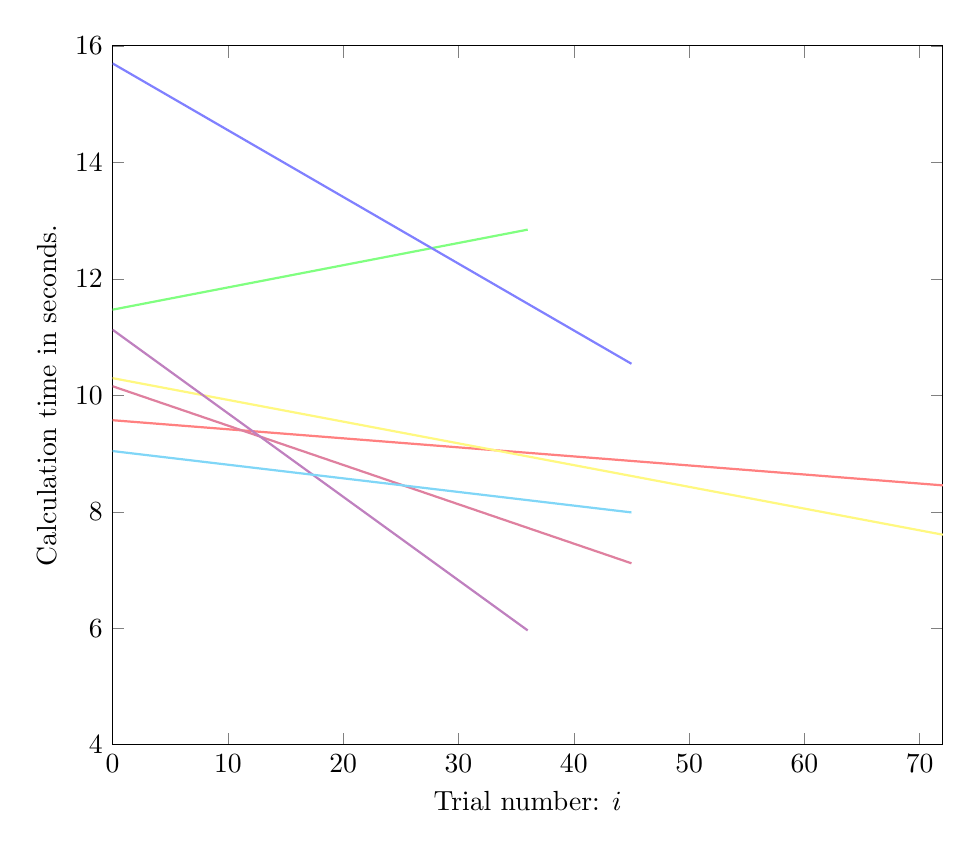
\begin{tikzpicture}
    \begin{axis}[
                enlargelimits=false,
                xlabel=Trial number: $i$,
                ylabel = Calculation time in seconds.,
                width=\textwidth,
                ymin=4,
                ymax=16
        ]
        \addplot[
            domain=0:72,
            samples=3,
            thick,
            color=red!50
        ]{9.572-0.015535*x};
        \addplot[
            domain=0:36,
            samples=3,
            thick,
            color=green!50
        ]{11.46978+0.03817*x};
        \addplot[
            domain=0:72,
            samples=3,
            thick,
            color=yellow!50
        ]{10.29454-0.037335*x};
        \addplot[
            domain=0:45,
            samples=3,
            thick,
            color=blue!50
        ]{15.6977-0.1146*x};
        \addplot[
            domain=0:45,
            samples=3,
            thick,
            color=purple!50
        ]{10.15532-0.06755*x};
        \addplot[
            domain=0:36,
            samples=3,
            thick,
            color=violet!50
        ]{11.12582-0.143408*x};
        \addplot[
            domain=0:45,
            samples=3,
            thick,
            color=cyan!50
        ]{9.04245-0.023411*x};
    \end{axis}

\end{tikzpicture}
\caption{Regression lines for the 7 participants with the most samples. A clear downward sloping trend in terms of calculation time is observed.}
\label{user-regression}
\end{figure}



\subsection{Failure rate.}
Failure rate is a key characteristic of the scheme. As mentioned it is essential that a user is able to calculate passwords correctly for the scheme to function. How high the failure rate can be depends on how long passwords are used and how often a user can enter the wrong password without locking the account. A typical password protected site will allow a minimum of three strikes before the account is locked~\cite{10-strikes}. It is thus important that the probability of being ``locked out'' is small enough for it not to happen often, how often is of course subject to discussion.

\begin{observation}\label{obs:failrate}
    Average failure rate for all samples recorded in the experiment was measured to be $\tilde \lambda = 0.0584795321637$, approximately every one out of 17 single digit challenge was calculated wrong.
\end{observation}
This observation might not seem very unusual, but since a password consists of a sequence of calculations, it is required that users calculate a given number of challenges consecutively without failure. It is thus more interesting to evaluate the probability of having at least one mistake in a complete password calculation sequence. It is also not unusual to enforce a password policy using a three-strike policy which locks the account if three consecutive mistakes are made. Next, these probabilities are presented and discussed. 


The probability of having at least one mistake in a length $l$ password given the failure rate $\lambda$ is given by
\begin{equation}\label{eq:failrate}
    P(fail) = 1 - (1 - \lambda)^l
\end{equation}

Next, the probability of getting the account locked given a three-strike policy with the same password and failure rate is 
\begin{equation}\label{eq:lockrate}
    P(lock) = ( 1 - (1 - \lambda)^l )^3
\end{equation}


\begin{table}[h]
    \centering
\begin{tabular}{|c|c|c|c|c|}
    \hline
    Password length $l$ & $3$ & $5$ & $10$ & $15$ \\ \hline \hline
    $P(fail)$ & $0.1654$ & $0.2601$ & $0.4526$ & $0.5959$ \\ \hline
    $P(lock)$ & $0.0045$ & $0.0176$ & $0.0927$ & $0.2107$ \\ \hline
\end{tabular}
\caption{Probability of having at least one mistake in a length $l$ password given failure rate $\lambda = 0.0584795321637$ for each single digit challenge.}
\label{tbl:failrate}
\end{table}
 
\par Observation \ref{tbl:failrate} shows the probabilities of calculating a password wrong once and three times in a row. If users want to use a password of 15 characters, which is reasonable to assume since the scheme only produce digits, they will compute a faulty password nearly 60\% of the time. This limits the usability severely, since users will more often than not, be unable to log in.
\par The probability of actually locking the account by miscalculating three passwords in a row, is lower but not significantly. With the same failure rate and password length, users would break the three-strike rule approximately one out of five login attempts.

\par To illustrate this consequence in a extreme case, consider the \emph{very active} user from table \ref{users} in section \ref{sec:usability} who visits 10 different accounts every day. Such an user would eventually lock two accounts every day with password lengths of 15 characters, which of course is not acceptable.

\par As discussed in \autoref{improving-usab} (and as implemented in \autoref{app}), the password length needed for different accounts may vary. By using shorter password for noncritical accounts, and only generating long passwords for the most critical, the average password length will be much lower than in the examples above. The scheme could then be tweaked by users to fit specific needs, instead of requiring 10 or 15 characters in all passwords generated. For less sensitive accounts users may have passwords of lengths 5, which would make for a mistake in approximately every 4th password, and only locking an account every 57th login attempt. This way users can calculate passwords with significantly less effort and lower failure rates. 

\par The experiment did not find any significant correlation between failure rates and calculation times. Users calculating fast do not have a higher failure rate than slower users, which some might expected. 

%\subsection{Improvement Measures.}
%\par Blocki et al.~\cite{hcp-blocki} suggests a tweak to the scheme with the purpose of decreasing the calculation time while still ensuring resistance against dictionary attacks. The suggestion is to memorize another mapping $w:\mathbb{Z}_{10} \rightarrow \{x\}$ with $x$ being one of the $10000$ most common English words. Then after computing $f(\sigma(C))$ the user would apply $w$ giving the corresponding word to the digit. The point of doing this is to save time when calculating, but it also solves the problem with high failure rates. Blocki argues, it would be sufficient with 3-5 challenges. With this assumption that 3-5 calculations are enough, the scheme would function significantly better. 
%\par Using the same example with the very active user, an account would be locked every 222nd login attempt with length 3 and every 57th with length 5. This would be a huge improvement, actually making the scheme usable.


\begin{remark}
    The author remarks that the findings related to failure rates might be too harsh since the participants was asked to calculate the challenges ``as fast as possible'', which might be the wrong approach. In a real world scenario it would be more important to calculate correctly. Though, the results clearly show that the failure rate is a relevant attribute worth investigating closer, as it might limit the reliability of the scheme in real usecases.
\end{remark}





\cleardoublepage
\chapter{Concluding Remarks and Further Work}
This project has presented the human computable password management scheme by Blocki et al.~\cite{hcp-blocki}, as well as the design and construction of two applications implementing the HCP scheme with different purposes. How different characteristic and parameters affect the usability of the scheme was discussed, as well as how password length and number of secret mappings affect the security. Failure rate was introduced as an important factor affecting the usability of the scheme. 
\par The first application is a Google Chrome browser extension, making it easy for users to employ the scheme without too much trouble. It is a fact that the scheme is quite complex and requires a lot dedication from the users for it to work. It is thus important to have a tool minimizing extra work required, including management and generation of challenges. Without a tool to take care of these obstacles, the scheme would be very hard to use in practice. With the application created in this project, users only have to worry about memorizing and rehearsing the secret mapping, all the overhead related to generation, storing and fetching of challenges is handled by the extension. The one choice users have to make is what category to put their accounts in, either low, medium or high sensitivity. This measure was introduced to increase the usability by lowering the average number of single digit challenges, while still keeping the important accounts secured.
\par The application is available in the browser, making it very accessible in situations where passwords are needed. The extension monitors the active page browsed by the users and fetches information from DOM allowing it to display the correct challenge at all times, both in regards to which page users are visiting and how many characters are entered in the password field. E.g. if users visit \url{google.com} the extension will get notice about this and bring up the challenges associated with \url{google.com}. If the site is not part of the system, users will get the chance to add it. When calculating passwords, the challenge on display update for each entered character in the password field.
\par The second application is a web application functioning as a demonstration platform as well as an experiment, gathering usage data. The experiment gathers data related to calculation time and failure rates. It was created to investigate how the scheme performs, with usability characteristics in focus. The participants in the experiment, gets a short introduction and the chance to practice until fairly familiar with the scheme. And are then asked to calculate a complete password consisting of 10 singlet digit challenges, while getting timed.
\par The experiment measured a average calculation time of $10.296$ seconds, with a standard deviation of $3.64$. This is considered to be reasonably good, as it should not limit the usability of the scheme severely. It could also be observed that users improved over time so that average calculation time would probably be even lower after some practice. 
\par A more unanticipated result was the failure rate, which was measured to be $0.058$, meaning that every 17 single digit challenge would be calculated wrong. This result should not be interpreted as a dismissal of the scheme, since different users will achieve different failure rates, and many will be able to calculate correctly most of the time. What should be emphasized though, is that the failure rate should be investigated closer, to verify that a general user average a low enough failure rate. 


\section{Further Work}

\subsection{Additional Applications.}
This project showed how browser extensions can be used to create an easy to used password management application. This choice was made with a goal of making a quite complex scheme usable without too much overhead and practice. To make the scheme even more accessible, it would be by creating an accompanying web application and possibly a mobile application. These applications could use the same storage, while still syncing to chrome storage for the browser extension and to mobile storage for the mobile application. It would be useful to have a user management page to overview user data and challenges. The construction presented here does not allow users to manually configure the account which some users might dislike. 

\subsection{Larger scale experiments}
It is, as mentioned, clear that the failure rate of the scheme is important for it to function in practice. The experiment conducted in this project did not aim to tell a truth or verify a hypothesis, which should be the next step. A typical setup would could be similar to the one presented here, but in a much larger scale, possibly using a crowd sourcing service or social media, asking the participants to calculate challenges. It would be important to get more samples from each participant, making it easier to calculate different averages after more practice.  
\par It would also be interesting to conduct a survey gathering data about how users rate their account. Typically asking how many they regard as ``highly sensitive'', ``don't-care'' etc. This would make it possible calculate an average password length which again could be used to measure failure rates and calculation times more thoroughly. By knowing how many account a user has of each type, it would be possible to say something about how many mappings would be sufficient to have in $\sigma$. 

\cleardoublepage
\renewcommand*{\bibname}{References}
\bibliographystyle{alpha}
\bibliography{main,biblo}







\appendix
\addtocontents{toc}{%
 \protect\vspace{1em}% 
 \protect\noindent \bfseries \appendixtocname\protect\par
 \protect\vspace{-.5em}%
}
\renewcommand{\chaptername}{\appendixname}

\chapter{Extension Class Files}\label{extension-classes}

\section{Content Script}\label{app:content-script}
\lstinputlisting[caption=Content script file., style=jsStyle, basicstyle=\scriptsize]{code/content_script.js}

The content script listens for the onload event triggered by the window object when a new page is loaded. When receiving this event the updateUrl function(line 29) is called, which sends an update containing  \emph{window.location.hostname} which is the hostname of the currently active page. Hostname is used since login forms may be located at different locations at different domains.
\par Next the script searches the DOM for input fields of type ``password'' using the \emph{getPwdInputs} function(line 18). This function iterates through all the input fields looking for password fields. If a password field is found, an event listener is attached to the field, listening for events of type ``input'' which are sent when the field changes\footnote{https://developer.mozilla.org/en-US/docs/Web/API/EventTarget/addEventListener}. When the password field changes a message containing the new length of the password is sent to the controller. 

\section{Controller}\label{app:controller}
\lstinputlisting[caption=Angular controller., style=jsStyle, basicstyle=\scriptsize]{code/controllers.js}
The controller is responsible for all the business logic, keeping the storage updated with new users and new sites. The \emph{newSite} method on line 11 is called when then ``new site''-button is clicked by the user, it then generates a new object of type Site with the domain name and selected site class (essentially the number of single digit challenges to be generated). The site is then added to the user object which is stored in the database to keep the storage persistent in case of disconnection. 
\par When the controller is loaded the first action executed is trying to load the user object from the storage (line 21), if no user object is found, the controller creates a new one. In the code presented here, a new user is initiated with a dummy site for demonstration purposes. All the storage specific methods are called from the \emph{chromeStorage} object, which makes it easy to do operations accessing the Chrome storage. The \emph{getOrElse} is used, which checks for a user object and creates a new if none is present. 
\par The controller also listens for messages from the content script, this event listener can be seen at line 62. When a message is received the \emph{handleMessage} is called to process the data, distinguishing between a changes in the URL and changes in password length. When data is received, the corresponding variable in the controller is updated. If a new site was added, the view is also updated, hiding the "new site"-button.

\section{App.js File}\label{app:app.js}
\lstinputlisting[caption=Angular launcher file., style=jsStyle, basicstyle=\scriptsize]{code/app.js}

The app.js file initiates the application, specifying the modules used, as well as some helper functions, including the function responsible for generating the random challenges(line 66). 

\section{View File (partial file)}\label{app:view}
\lstinputlisting[caption=Angular view. Only included the table showing the challenges for readability., style=jsStyle, basicstyle=\scriptsize, firstline=12, lastline=91]{code/content.html}
The code shown in this listing contains the view where the challenges are presented, as well as the new site button and site classification radio buttons. Notice the \emph{ng-show} directive on line 14, this decides if the "new site"-functionality should be shown or not. If \emph{newSiteButton} is true it will appearer and vice versa, the same goes for the challenges which starts on line 34 with a similar directive, \emph{ng-hide}, which hides the challenges div if new site is visible.  
\par The challenges div is essentially a table containing an element of the challenge in each cell. Notice the double bracket notation, where each of the challenge objects are referred. \emph{\{\{site.challenges[pw][i]\}\}} refers to the \emph{\$scope.site.challenges} which contains the challenges associated with the current active page. $pw$ is at any given time the length of the password field of the active web page, if $pw$ changes the challenge on display will automatically change through the two-way data binding. This way, the correct challenge will always be the one seen by the user.


\chapter{Demonstration Slides}\label{demo-slides}

\begin{figure}
    \includegraphics[width=\textwidth]{slides/slide1}
    \caption{Demo slide 1.}
    \label{slide1}
\end{figure}


\begin{figure}
    \includegraphics[width=\textwidth]{slides/slide2}
    \caption{Demo slide 2.}
    \label{slide2}
\end{figure}


\begin{figure}
    \includegraphics[width=\textwidth]{slides/slide3}
    \caption{Demo slide 3.}
    \label{slide3}
\end{figure}


\begin{figure}
    \includegraphics[width=\textwidth]{slides/slide4}
    \caption{Demo slide 4.}
    \label{slide4}
\end{figure}

\begin{figure}
    \includegraphics[width=\textwidth]{slides/slide5}
    \caption{Demo slide 5.}
    \label{slide5}
\end{figure}


\begin{figure}
    \includegraphics[width=\textwidth]{slides/slide6}
    \caption{Demo slide 6.}
    \label{slide6}
\end{figure}

\cleardoublepage




\chapter{Experiment Application}\label{experiment-views}

\begin{figure}
    \includegraphics[width=\textwidth]{view1}
    \caption{First view shown to the user, containing a demonstration video. Created using \url{wideo.co}.}
    \label{view1}
\end{figure}

\begin{figure}
    \includegraphics[width=\textwidth]{view2}
    \caption{Second view shown to the user, gathering some basic demographic data which might be relevant. }
    \label{view2}
\end{figure}

\begin{figure}
    \includegraphics[width=\textwidth]{view3}
    \caption{Third view of the web application. Practice section used by the user before entering the actual experiment.}
    \label{view3}
\end{figure}

\begin{figure}
    \includegraphics[width=\textwidth]{view4}
    \caption{Final view, containing the experiment form. The user will calculate the response to the challenge on display and enter the answer in the password field. When finished the results can be submitted. And eventually stored in the database.}
    \label{view4}
\end{figure}



\end{document} 
